\documentclass{beamer}
\usepackage{listings}
\usepackage{graphicx}
\usepackage{bm}
\usepackage{amsmath,amssymb,xcolor,graphicx,url,natbib}
\usepackage{amsthm}
\usepackage{subfigure} % allow matrices of figures
\bibliographystyle{abbrv}
\usepackage{float}
\usepackage{animate}
\usepackage{pgffor}
\usepackage{hyperref}
\usepackage{mathrsfs}
\usepackage[absolute,overlay]{textpos}


\newcommand{\bd}{\begin{description}} 
\newcommand{\ed}{\end{description}} 
\newcommand{\bi}{\begin{itemize}} 
\newcommand{\ei}{\end{itemize}} 

%\logo{
\includegraphics[width=2cm]{plots/TAB_col_white_background.eps}}

%\addtobeamertemplate{frametitle}{}{
%	\vspace{-0.6cm}\hfill\raisebox{-0.65ex}{
\includegraphics[height=1cm]{plots/TAB_col_white_background.eps}}}

\usepackage{tikz}

\addtobeamertemplate{frametitle}{}{
	\begin{tikzpicture}[remember picture,overlay]
		\node[anchor=north east, xshift=0.05cm, yshift=0cm] at (current page.north east)
		{
\includegraphics[height=1cm]{plots/TAB_col_white_background.eps}};
	\end{tikzpicture}
}


\setbeamertemplate{footline}{\scriptsize
	\hfill \insertframenumber
}


\title{\fontsize{14pt}{12pt}\selectfont Elastic fibres in shear flows can maintain steady orientations}
%\subtitle{}
\author{
	Hao Ye \\ \textit{Department of Mathematics} \\
	\vspace{0.5cm} 
	Supervisors: \\Matthias Heil, Draga Pihler-Puzović
}
%\date{\tiny Please update course code, project number, name and Student ID!}
\begin{document}

\begin{frame}[plain] 
	\maketitle 
	
	%\vfill 
	
	\begin{center}
		
\includegraphics[height=1.2cm]{plots/TAB_col_white_background.eps} 
	\end{center}
\end{frame}

%%%%%%%%%%%%%%%%%%%%%%%%%%%%%%%%%%%%%%%%%%%%%%%%%%%%%%%%%%%%%%%%%%%%%%

%\frame{\titlepage}

%%%%%%%%%%%%%%%%%%%%%%%%%%%%%%%%%%%%%%%%%%%%%%%%%%%%%%%%%%%%%%%%%%%%%%

\begin{frame}
	\frametitle{Motivation: particles/fibres in shear flow}
	\begin{overlayarea}{\textwidth}{\textheight}
		\vspace{-0.2cm}
    	\begin{figure}
			\begin{minipage}{0.4\linewidth}
				\centering
				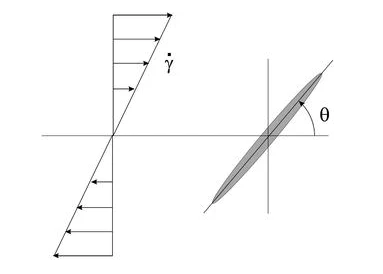
\includegraphics[width=\linewidth]{plots/application2.png} 
			 \centering \scriptsize A rigid ellipsoid \cite{yasuda2004experimental}.
			\end{minipage}
		\begin{minipage}{0.5\linewidth}
			\centering
			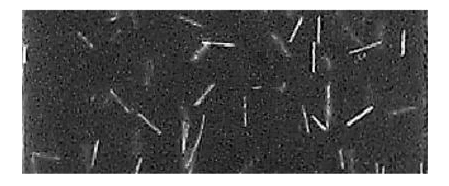
\includegraphics[width=\linewidth]{plots/application2_2.png} 
			\centering \scriptsize Vinylon fibers (paper industry) \cite{yasuda2004experimental}.
		\end{minipage}\vspace{0.5cm}
	\begin{minipage}{0.3\linewidth}
		\centering
		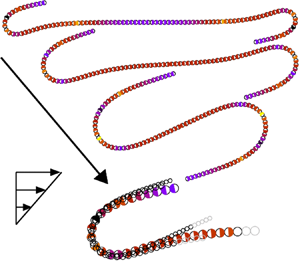
\includegraphics[width=\linewidth]{plots/application6.png} 
		\centering \scriptsize Elongated elastic fibres \cite{zuk2021universal}.
	\end{minipage}
		\begin{minipage}{0.32\linewidth}
		\centering
		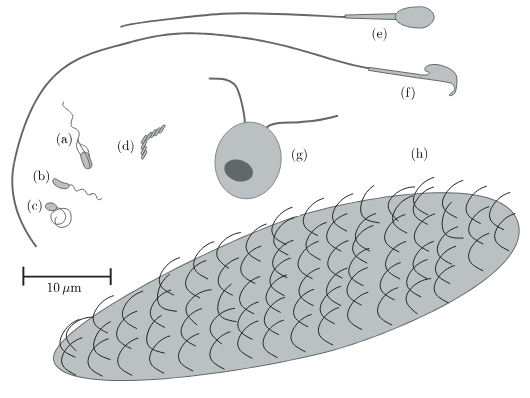
\includegraphics[width=\linewidth]{plots/application1.png} 
		\centering \scriptsize Sketches of microscopic swimmers, to scale \cite{lauga2009hydrodynamics}.
	\end{minipage}
		\begin{minipage}{0.35\linewidth}
	\centering
	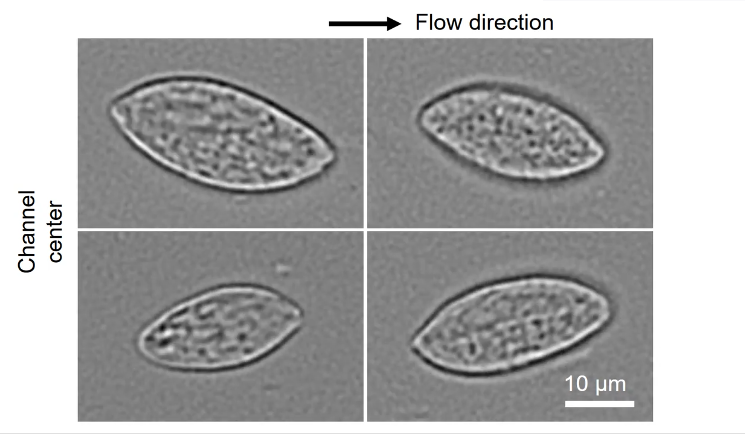
\includegraphics[width=\linewidth]{plots/application5.png}
	\centering \scriptsize Tank-treading motion of cells (video) \cite{gerum2022viscoelastic}.
\end{minipage}
		\end{figure}
	\end{overlayarea}
\end{frame}

%%%%%%%%%%%%%%%%%%%%%%%%%%%%%%%%%%%%%%%%%%%%%%%%%%%%%%%%%%%%%%%%%%%%%%

\begin{frame}
	\frametitle{Introduction: Jeffery orbits}
	\begin{overlayarea}{\textwidth}{\textheight}
		\vspace{-0.2cm}
	\begin{columns}
	\column{.6\textwidth}
	\begin{figure}[htb]
		\begin{center}
			% specify width as 80% of the width of the text on the page
			% we can also specify a width in centimetres, e.g. [width=8cm]
			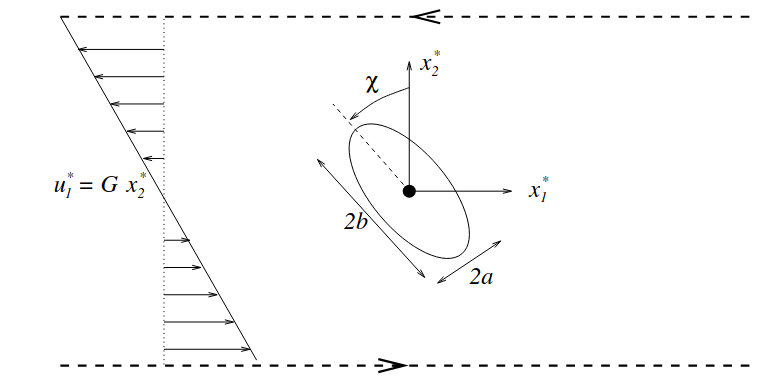
\includegraphics[width=1\textwidth]{plots/jeffery.png}
		\end{center}
		%	\setlength{\abovecaptionskip}{-0.5 cm}
	\end{figure}
	\column{.55\textwidth}
	\small
	\bi
	\item Jeffery (1922): periodic tumbling motion of rigid ellipsoidal particles in shear flow.
	\ei 
\end{columns}
\vspace{0.5cm}
\bi 
\item If vorticity $\omega\neq 0$, typically particles will undergo a periodic rotation (Jeffery orbits).
	\item The periodic motion depends on the particle shapes ($\&$ initial conditions).
\ei
		%\vspace{0.1cm}
	\end{overlayarea}
\end{frame}


%%%%%%%%%%%%%%%%%%%%%%%%%%%%%%%%%%%%%%%%%%%%%%%%%%%%%%%%%%%%%%%%%%%%%%

\begin{frame}
	\frametitle{Introduction: Jeffery orbits}
	\begin{overlayarea}{\textwidth}{\textheight}
		\vspace{-0.2cm}
		\begin{columns}
			\column{.6\textwidth}
			\begin{figure}[htb]
				\begin{center}
					% specify width as 80% of the width of the text on the page
					% we can also specify a width in centimetres, e.g. [width=8cm]
					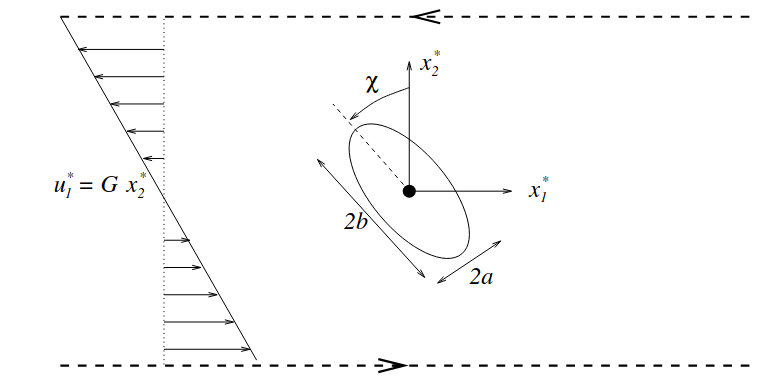
\includegraphics[width=1\textwidth]{plots/jeffery.png}
				\end{center}
				%	\setlength{\abovecaptionskip}{-0.5 cm}
			\end{figure}
			\column{.55\textwidth}
			\small
			\bi
			\item Jeffery (1922): periodic tumbling motion of rigid ellipsoidal particles in shear flow.
			\ei 
		\end{columns}
		\vspace{0.5cm}
		\bi 
		\item If vorticity $\omega\neq 0$, typically particles will undergo a periodic rotation (Jeffery orbits).
		\item The periodic motion depends on the particle shapes ($\&$ initial conditions).
		\item \alert{Some exceptions for esoteric shapes} (Brenner (1963)). No rotation!
		\ei

		%\vspace{0.1cm}
	\end{overlayarea}
\end{frame}

%%%%%%%%%%%%%%%%%%%%%%%%%%%%%%%%%%%%%%%%%%%%%%%%%%%%%%%%%%%%%%%%%%%%%%


\begin{frame}
	\frametitle{Our interest: Boomerang-shaped rigid fibres}
	\begin{overlayarea}{\textwidth}{\textheight}
		\vspace{-0.5cm}\footnotesize Roggeveen J V, Stone H A. JFM (2022), 939: A23.\vspace{-0.2cm}
		\begin{figure}[htb]
			\begin{center}
				% specify width as 80% of the width of the text on the page
				% we can also specify a width in centimetres, e.g. [width=8cm]
				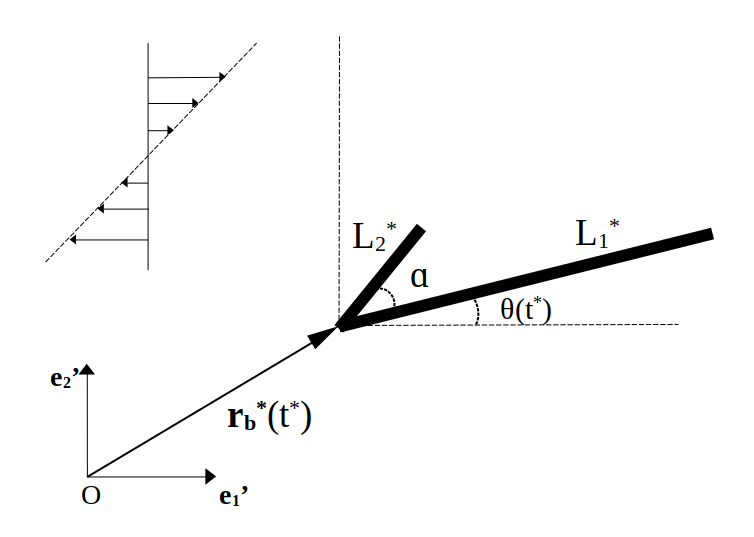
\includegraphics[width=0.6\textwidth]{plots/schematic/schematic_rigid_configuration.png}
			\end{center}
			%	\setlength{\abovecaptionskip}{-0.5 cm}
		\end{figure}\vspace{-0.3cm}
     	\small \bi
		\item Opening angle $\alpha$. 
		\item Length $L_1^*,L_2^*$: $\mathcal{L}=L_1^*+L_2^*;\, L_{1,2}^*=\mathcal{L}(\frac{1}{2}\pm q)$, $q$ is "aspect ratio".
	    \item As $q$ increases, the short arm shortens while the long arm lengthens.
	    \ei 
	\end{overlayarea}
\end{frame}


%%%%%%%%%%%%%%%%%%%%%%%%%%%%%%%%%%%%%%%%%%%%%%%%%%%%%%%%%%%%%%%%%%%%%%


\begin{frame}
	\frametitle{Our interest: Boomerang-shaped rigid fibres}
	\begin{overlayarea}{\textwidth}{\textheight}
		\vspace{-0.5cm}\footnotesize Roggeveen J V, Stone H A. JFM (2022), 939: A23.\vspace{-0.2cm}
		\begin{figure}[htb]
			\begin{center}
				% specify width as 80% of the width of the text on the page
				% we can also specify a width in centimetres, e.g. [width=8cm]
				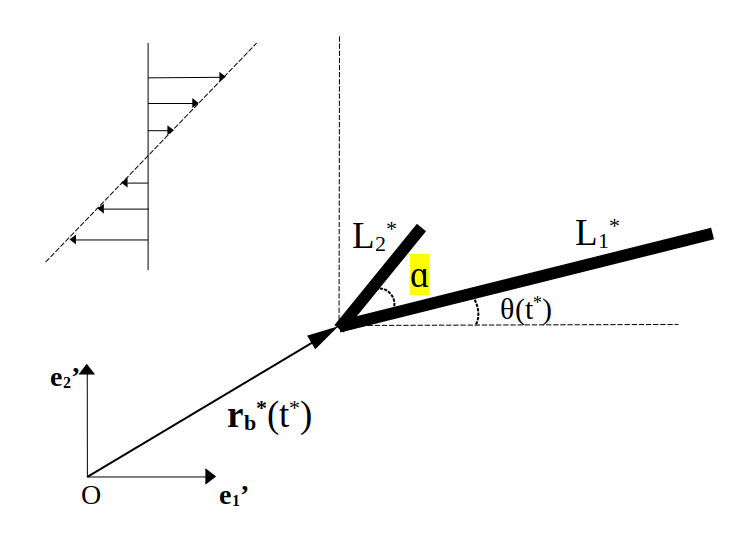
\includegraphics[width=0.6\textwidth]{plots/schematic/schematic_rigid_configuration_alpha.png}
			\end{center}
			%	\setlength{\abovecaptionskip}{-0.5 cm}
		\end{figure}\vspace{-0.3cm}
		\small \bi
		\item \colorbox{yellow}{Opening angle $\alpha$}. 
		\item Length $L_1^*,L_2^*$: $\mathcal{L}=L_1^*+L_2^*;\, L_{1,2}^*=\mathcal{L}(\frac{1}{2}\pm q)$, $q$ is "aspect ratio".
		\item As $q$ increases, the short arm shortens while the long arm lengthens.
		\ei 
	\end{overlayarea}
\end{frame}


%%%%%%%%%%%%%%%%%%%%%%%%%%%%%%%%%%%%%%%%%%%%%%%%%%%%%%%%%%%%%%%%%%%%%%


\begin{frame}
	\frametitle{Our interest: Boomerang-shaped rigid fibres}
	\begin{overlayarea}{\textwidth}{\textheight}
		\vspace{-0.5cm}\footnotesize Roggeveen J V, Stone H A. JFM (2022), 939: A23.\vspace{-0.2cm}
		\begin{figure}[htb]
			\begin{center}
				% specify width as 80% of the width of the text on the page
				% we can also specify a width in centimetres, e.g. [width=8cm]
				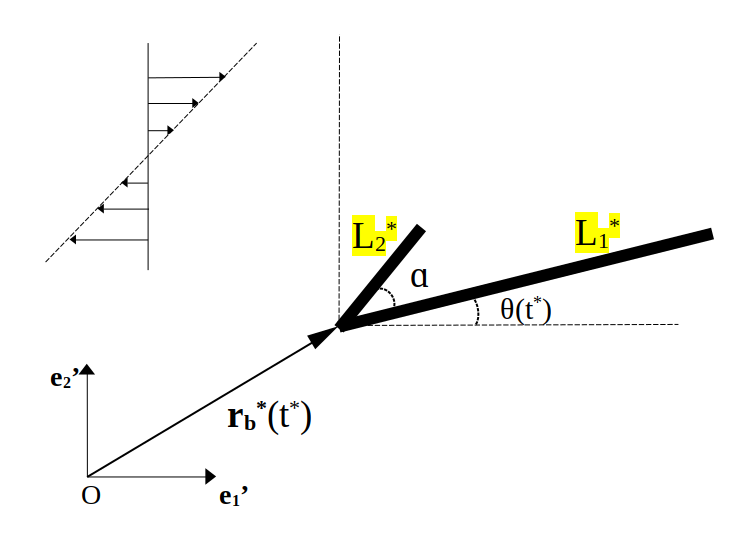
\includegraphics[width=0.6\textwidth]{plots/schematic/schematic_rigid_configuration_q.png}
			\end{center}
			%	\setlength{\abovecaptionskip}{-0.5 cm}
		\end{figure}\vspace{-0.3cm}
		\small \bi
		\item Opening angle $\alpha$. 
		\item Length $L_1^*,L_2^*$: $\mathcal{L}=L_1^*+L_2^*;\, L_{1,2}^*=\mathcal{L}(\frac{1}{2}\pm q)$, \colorbox{yellow}{$q$ is "aspect ratio"}.
		\item As $q$ increases, the short arm shortens while the long arm lengthens.
		\ei 
	\end{overlayarea}
\end{frame}


%%%%%%%%%%%%%%%%%%%%%%%%%%%%%%%%%%%%%%%%%%%%%%%%%%%%%%%%%%%%%%%%%%%%%%

\begin{frame}
	\frametitle{Our interest: Boomerang-shaped rigid fibres}
	\begin{overlayarea}{\textwidth}{\textheight}
		\vspace{-0.5cm}\footnotesize Roggeveen J V, Stone H A. JFM (2022), 939: A23.\vspace{-0.2cm}
		\begin{figure}[htb]
			\begin{center}
				% specify width as 80% of the width of the text on the page
				% we can also specify a width in centimetres, e.g. [width=8cm]
				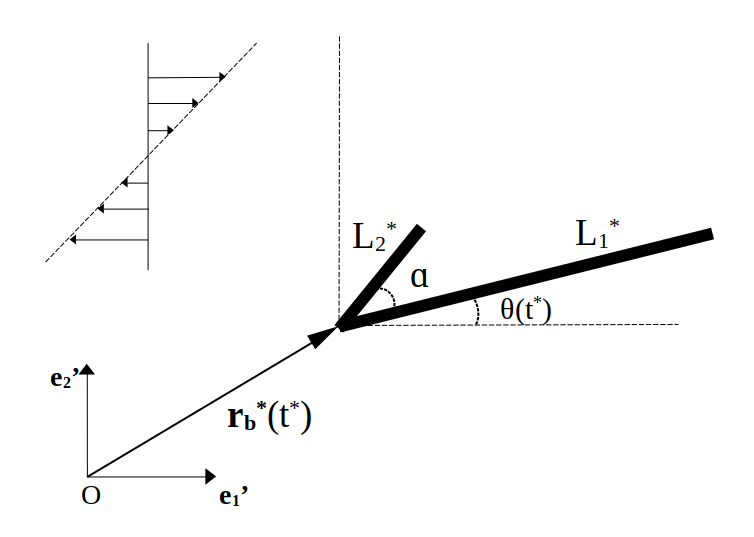
\includegraphics[width=0.6\textwidth]{plots/schematic/schematic_rigid_configuration.png}
			\end{center}
			%	\setlength{\abovecaptionskip}{-0.5 cm}
		\end{figure}\vspace{-0.3cm}
		\small \bi
		\item Opening angle $\alpha$. 
		\item Length $L_1^*,L_2^*$: $\mathcal{L}=L_1^*+L_2^*;\, L_{1,2}^*=\mathcal{L}(\frac{1}{2}\pm q)$, $q$ is "aspect ratio".
		\item As $q$ increases, the short arm shortens while the long arm lengthens.
		\item \colorbox{yellow}{For certain ranges of $(\alpha,q)$, these fibres don't rotate}.
		\ei 
	\end{overlayarea}
\end{frame}


%%%%%%%%%%%%%%%%%%%%%%%%%%%%%%%%%%%%%%%%%%%%%%%%%%%%%%%%%%%%%%%%%%%%%%

\begin{frame}
	\frametitle{Theory: slender body theory (SBT)}
	\begin{overlayarea}{\textwidth}{\textheight}
		\vspace{-0.5cm}\small Roggeveen $\&$ Stone described the motion by SBT. \normalsize 
		\begin{columns}
			\column{.6\textwidth}	
			\begin{figure}[htb]
				\begin{center}
					% specify width as 80% of the width of the text on the page
					% we can also specify a width in centimetres, e.g. [width=8cm]
					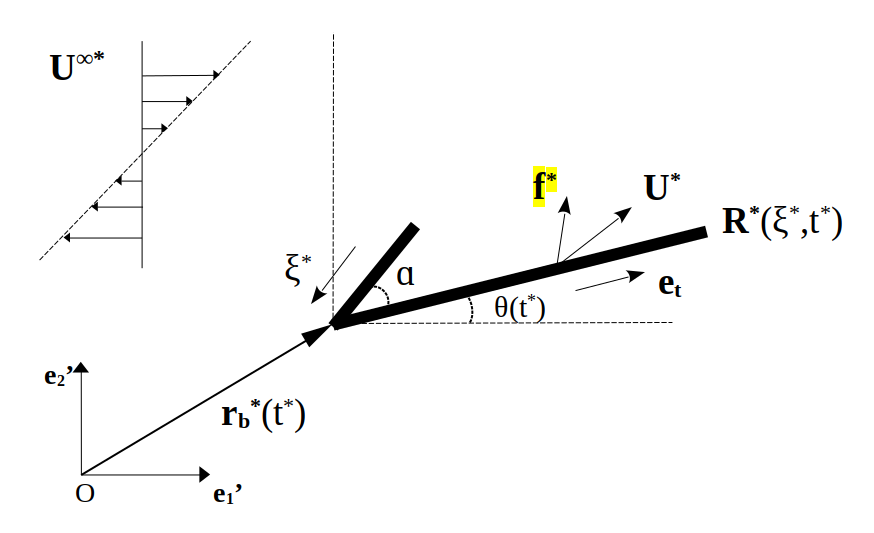
\includegraphics[width=1\textwidth]{plots/schematic/schematic_rigid_configuration_color0.png}
				\end{center}
				%	\setlength{\abovecaptionskip}{-0.5 cm}
			\end{figure}
			\column{.57\textwidth}
		\end{columns}\vspace{0.5cm}
		The local fluid traction on the fibre is given by: 
		\begin{equation*}
			\colorbox{yellow}{$\mathbf{f}^*$}=c_\perp\left(\mathbf{I}-\frac{1}{2}\mathbf{e}_t\mathbf{e}_t\right)\cdot(\mathbf{U}^{\infty*}-\mathbf{U}^*).
		\end{equation*}
	\end{overlayarea}
\end{frame}

%%%%%%%%%%%%%%%%%%%%%%%%%%%%%%%%%%%%%%%%%%%%%%%%%%%%%%%%%%%%%%%%%%%%%%


\begin{frame}
	\frametitle{Theory: slender body theory (SBT)}
	\begin{overlayarea}{\textwidth}{\textheight}
	\vspace{-0.5cm}\small Roggeveen $\&$ Stone described the motion by SBT. \normalsize 
		\begin{columns}
			\column{.6\textwidth}	
			\begin{figure}[htb]
				\begin{center}
					% specify width as 80% of the width of the text on the page
					% we can also specify a width in centimetres, e.g. [width=8cm]
					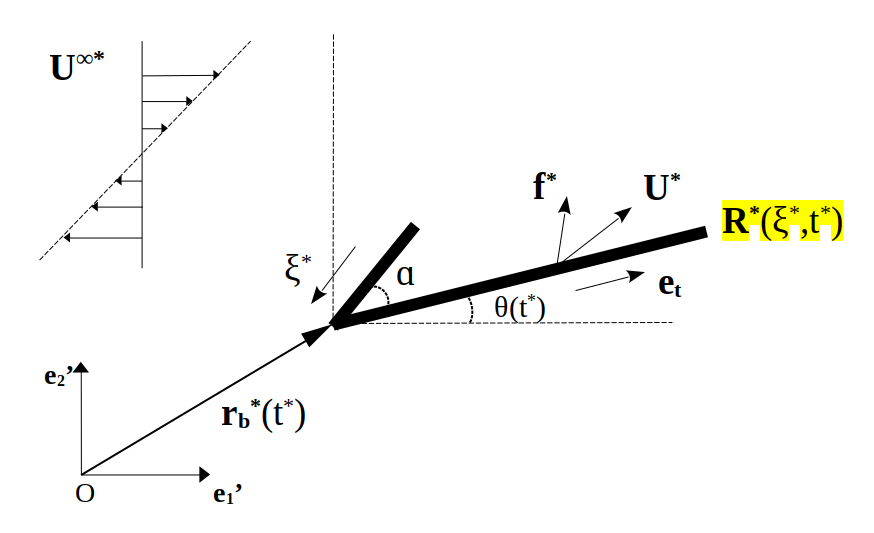
\includegraphics[width=1\textwidth]{plots/schematic/schematic_rigid_configuration_color1.png}
				\end{center}
				%	\setlength{\abovecaptionskip}{-0.5 cm}
			\end{figure}
			\column{.57\textwidth}
			\small \bi 
			\item \colorbox{yellow}{$\mathbf{R}^*(\xi^*,t^*)$}: particle geometry.
			\item $\theta(t^*)$: particle orientation.
			\item $\mathbf{e}_t$: tangent to the surface of particle.
			\item $\mathbf{U}^{\infty*}$: velocity of background flow.
			\item $\mathbf{U}^*$: local $\&$ instantaneous velocity of particle.
			\ei
		\end{columns}\vspace{0.5cm}
		The local fluid traction on the fibre is given by: 
		\begin{equation*}
			\mathbf{f}^*=c_\perp\left(\mathbf{I}-\frac{1}{2}\mathbf{e}_t\mathbf{e}_t\right)\cdot(\mathbf{U}^{\infty*}-\mathbf{U}^*).
		\end{equation*}
	\end{overlayarea}
\end{frame}

%%%%%%%%%%%%%%%%%%%%%%%%%%%%%%%%%%%%%%%%%%%%%%%%%%%%%%%%%%%%%%%%%%%%%%


\begin{frame}
	\frametitle{Theory: slender body theory (SBT)}
	\begin{overlayarea}{\textwidth}{\textheight}
		\vspace{-0.5cm}\small Roggeveen $\&$ Stone described the motion by SBT. \normalsize
		\begin{columns}
			\column{.6\textwidth}	
			\begin{figure}[htb]
				\begin{center}
					% specify width as 80% of the width of the text on the page
					% we can also specify a width in centimetres, e.g. [width=8cm]
					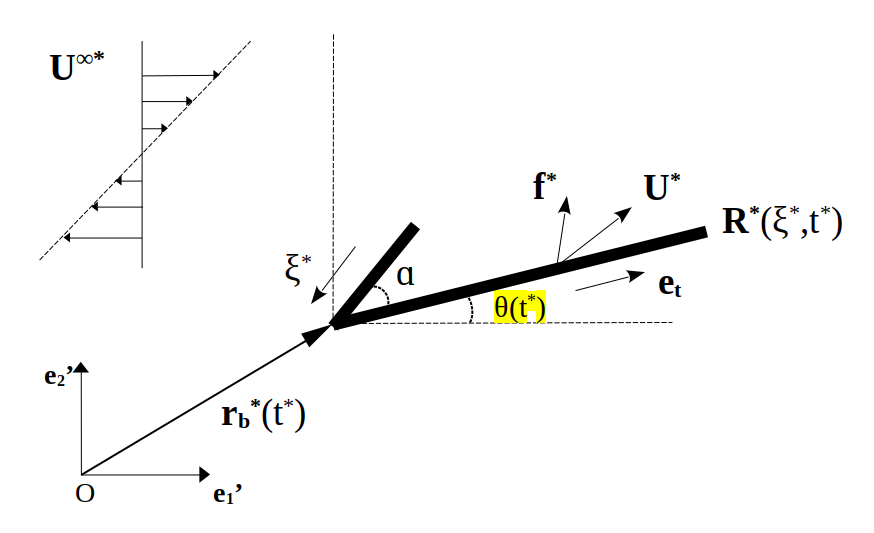
\includegraphics[width=1\textwidth]{plots/schematic/schematic_rigid_configuration_color2.png}
				\end{center}
				%	\setlength{\abovecaptionskip}{-0.5 cm}
			\end{figure}
			\column{.57\textwidth}
			\small \bi 
			\item $\mathbf{R}^*(\xi^*,t^*)$: particle geometry.
			\item \colorbox{yellow}{$\theta(t^*)$}: particle orientation.
			\item $\mathbf{e}_t$: tangent to the surface of particle.
			\item $\mathbf{U}^{\infty*}$: velocity of background flow.
			\item $\mathbf{U}^*$: local $\&$ instantaneous velocity of particle.
			\ei
		\end{columns}\vspace{0.5cm}
	The local fluid traction on the fibre is given by: 
		\begin{equation*}
			\mathbf{f}^*=c_\perp\left(\mathbf{I}-\frac{1}{2}\mathbf{e}_t\mathbf{e}_t\right)\cdot(\mathbf{U}^{\infty*}-\mathbf{U}^*).
		\end{equation*}
	\end{overlayarea}
\end{frame}

%%%%%%%%%%%%%%%%%%%%%%%%%%%%%%%%%%%%%%%%%%%%%%%%%%%%%%%%%%%%%%%%%%%%%%


\begin{frame}
	\frametitle{Theory: slender body theory (SBT)}
	\begin{overlayarea}{\textwidth}{\textheight}
		\vspace{-0.5cm}\small Roggeveen $\&$ Stone described the motion by SBT. \normalsize
		\begin{columns}
			\column{.6\textwidth}	
			\begin{figure}[htb]
				\begin{center}
					% specify width as 80% of the width of the text on the page
					% we can also specify a width in centimetres, e.g. [width=8cm]
					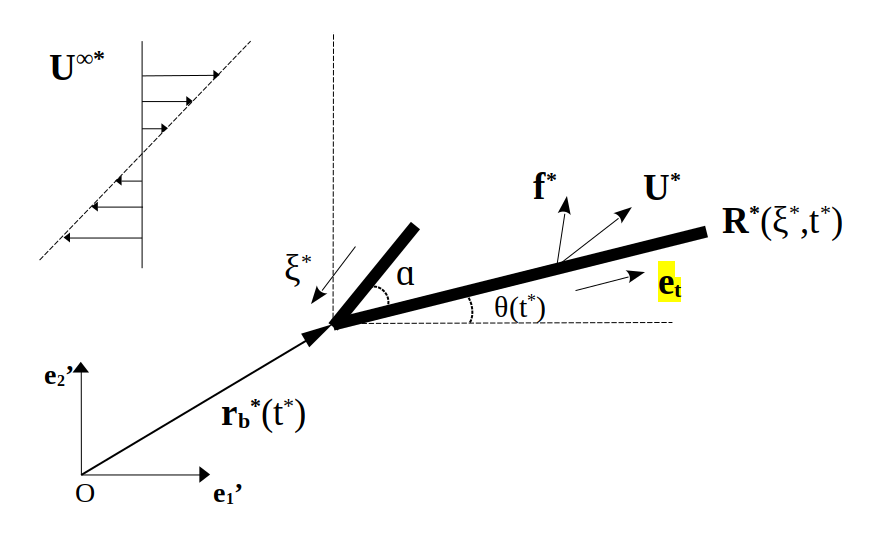
\includegraphics[width=1\textwidth]{plots/schematic/schematic_rigid_configuration_color3.png}
				\end{center}
				%	\setlength{\abovecaptionskip}{-0.5 cm}
			\end{figure}
			\column{.57\textwidth}
			\small \bi 
			\item $\mathbf{R}^*(\xi^*,t^*)$: particle geometry.
			\item $\theta(t^*)$: particle orientation.
			\item \colorbox{yellow}{$\mathbf{e}_t$}: tangent to the surface of particle.
			\item $\mathbf{U}^{\infty*}$: velocity of background flow.
			\item $\mathbf{U}^*$: local $\&$ instantaneous velocity of particle.
			\ei
		\end{columns}\vspace{0.5cm}
	The local fluid traction on the fibre is given by: 
		\begin{equation*}
			\mathbf{f}^*=c_\perp\left(\mathbf{I}-\frac{1}{2}\colorbox{yellow}{$\mathbf{e}_t\mathbf{e}_t$}\right)\cdot(\mathbf{U}^{\infty*}-\mathbf{U}^*).
		\end{equation*}
	\end{overlayarea}
\end{frame}

%%%%%%%%%%%%%%%%%%%%%%%%%%%%%%%%%%%%%%%%%%%%%%%%%%%%%%%%%%%%%%%%%%%%%%


\begin{frame}
	\frametitle{Theory: slender body theory (SBT)}
	\begin{overlayarea}{\textwidth}{\textheight}
		\vspace{-0.5cm}\small Roggeveen $\&$ Stone described the motion by SBT. \normalsize
		\begin{columns}
			\column{.6\textwidth}	
			\begin{figure}[htb]
				\begin{center}
					% specify width as 80% of the width of the text on the page
					% we can also specify a width in centimetres, e.g. [width=8cm]
					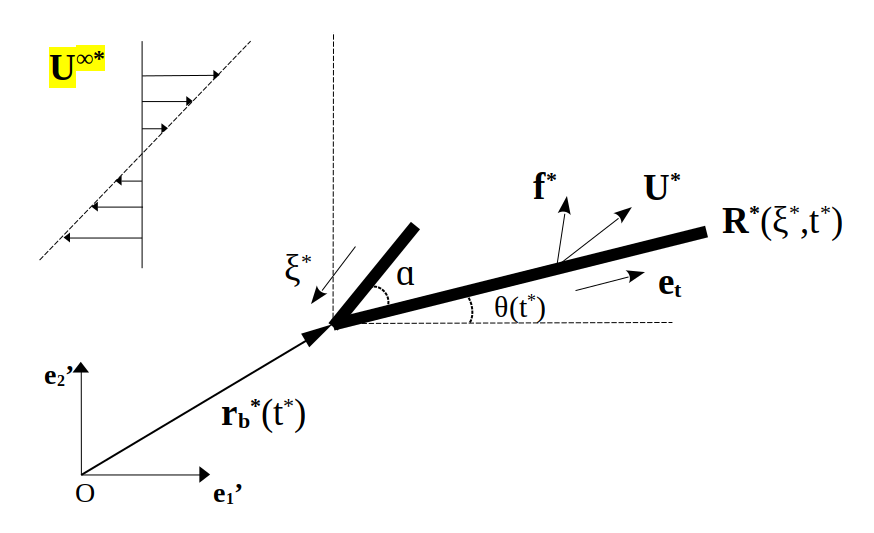
\includegraphics[width=1\textwidth]{plots/schematic/schematic_rigid_configuration_color4.png}
				\end{center}
				%	\setlength{\abovecaptionskip}{-0.5 cm}
			\end{figure}
			\column{.57\textwidth}
			\small \bi 
			\item $\mathbf{R}^*(\xi^*,t^*)$: particle geometry.
			\item $\theta(t^*)$: particle orientation.
			\item $\mathbf{e}_t$: tangent to the surface of particle.
			\item \colorbox{yellow}{$\mathbf{U}^{\infty*}$}: velocity of background flow.
			\item $\mathbf{U}^*$: local $\&$ instantaneous velocity of particle.
			\ei
		\end{columns}\vspace{0.5cm}
	The local fluid traction on the fibre is given by: 
		\begin{equation*}
			\mathbf{f}^*=c_\perp\left(\mathbf{I}-\frac{1}{2}\mathbf{e}_t\mathbf{e}_t\right)\cdot(\colorbox{yellow}{$\mathbf{U}^{\infty*}$}-\mathbf{U}^*).
		\end{equation*}
	\end{overlayarea}
\end{frame}

%%%%%%%%%%%%%%%%%%%%%%%%%%%%%%%%%%%%%%%%%%%%%%%%%%%%%%%%%%%%%%%%%%%%%%

\begin{frame}
	\frametitle{Theory: slender body theory (SBT)}
	\begin{overlayarea}{\textwidth}{\textheight}
		\vspace{-0.5cm}\small Roggeveen $\&$ Stone described the motion by SBT. \normalsize
		\begin{columns}
			\column{.6\textwidth}	
			\begin{figure}[htb]
				\begin{center}
					% specify width as 80% of the width of the text on the page
					% we can also specify a width in centimetres, e.g. [width=8cm]
					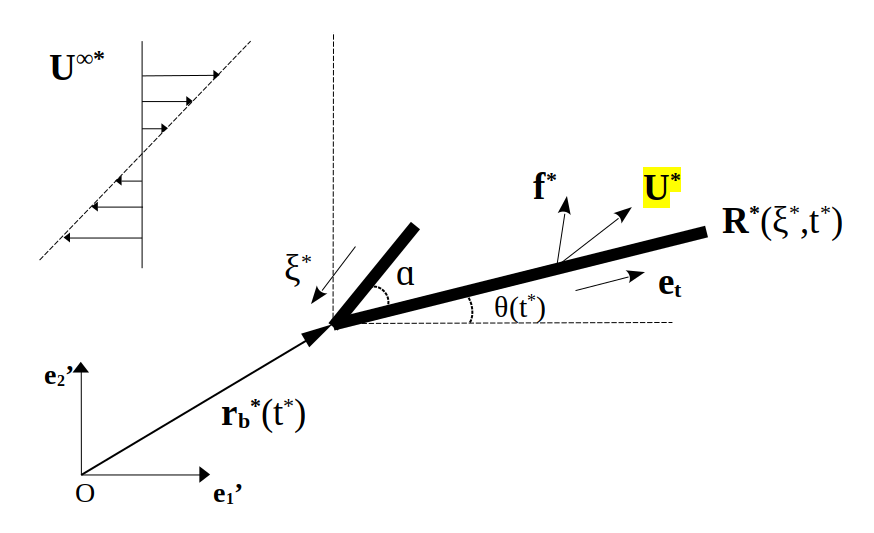
\includegraphics[width=1\textwidth]{plots/schematic/schematic_rigid_configuration_color5.png}
				\end{center}
				%	\setlength{\abovecaptionskip}{-0.5 cm}
			\end{figure}
			\column{.57\textwidth}
			\small \bi 
			\item $\mathbf{R}^*(\xi^*,t^*)$: particle geometry.
			\item $\theta(t^*)$: particle orientation.
			\item $\mathbf{e}_t$: tangent to the surface of particle.
			\item $\mathbf{U}^{\infty*}$: velocity of background flow.
			\item \colorbox{yellow}{$\mathbf{U}^*$}: local $\&$ instantaneous velocity of particle.
			\ei
		\end{columns}\vspace{0.5cm}
		The local fluid traction on the fibre is given by: 
		\begin{equation*}
			\mathbf{f}^*=c_\perp\left(\mathbf{I}-\frac{1}{2}\mathbf{e}_t\mathbf{e}_t\right)\cdot(\mathbf{U}^{\infty*}-\colorbox{yellow}{$\mathbf{U}^*$}).
		\end{equation*}
	\end{overlayarea}
\end{frame}

%%%%%%%%%%%%%%%%%%%%%%%%%%%%%%%%%%%%%%%%%%%%%%%%%%%%%%%%%%%%%%%%%%%%%%

\begin{frame}
	\frametitle{How to find non-rotating configurations?}
	\begin{overlayarea}{\textwidth}{\textheight}
		\vspace{-0.6cm}
		\begin{columns}
			\column{.65\textwidth}	
			\begin{figure}[htb]
				\begin{center}
					% specify width as 80% of the width of the text on the page
					% we can also specify a width in centimetres, e.g. [width=8cm]
					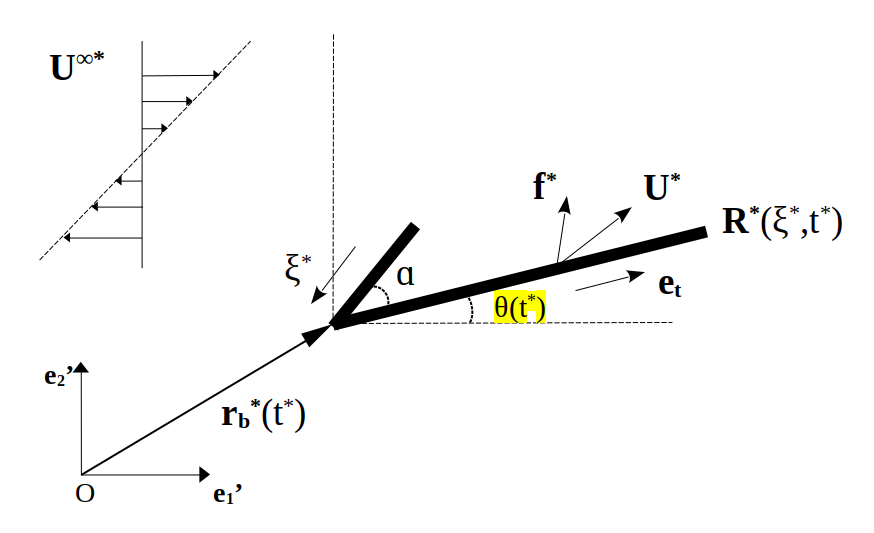
\includegraphics[width=0.8\textwidth]{plots/schematic/schematic_rigid_configuration_color2.png}
				\end{center}
				%	\setlength{\abovecaptionskip}{-0.5 cm}
			\end{figure}\vspace{0.3cm}
			\column{.5\textwidth}
			\small 	The local fluid traction on the fibre is given by: 
			\begin{equation*}
				\mathbf{f}^*=c_\perp\left(\mathbf{I}-\frac{1}{2}\mathbf{e}_t\mathbf{e}_t\right)\cdot(\mathbf{U}^{\infty*}-\mathbf{U}^*).
			\end{equation*}
		\end{columns}\vspace{-0.5cm}
		\begin{columns}
			\column{.58\textwidth}	
			\column{.58\textwidth} \vspace{-0.1cm}
		\end{columns}
	\vspace{0.5cm}
		%\selectfont \fontsize{10}{15}\selectfont
	\end{overlayarea}
\end{frame}

%%%%%%%%%%%%%%%%%%%%%%%%%%%%%%%%%%%%%%%%%%%%%%%%%%%%%%%%%%%%%%%%%%%%%%

\begin{frame}
	\frametitle{How to find non-rotating configurations?}
	\begin{overlayarea}{\textwidth}{\textheight}
		\vspace{-0.6cm}
		\begin{columns}
			\column{.65\textwidth}	
			\begin{figure}[htb]
				\begin{center}
					% specify width as 80% of the width of the text on the page
					% we can also specify a width in centimetres, e.g. [width=8cm]
					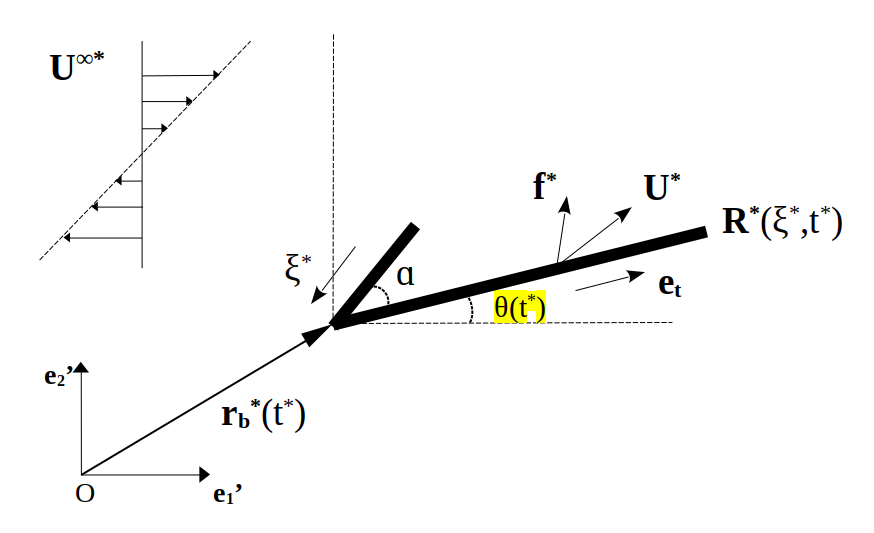
\includegraphics[width=0.8\textwidth]{plots/schematic/schematic_rigid_configuration_color2.png}
				\end{center}
				%	\setlength{\abovecaptionskip}{-0.5 cm}
			\end{figure}\vspace{0.3cm}
			\column{.5\textwidth}
			\small The local fluid traction on the fibre is given by: 
			\begin{equation*}
				\mathbf{f}^*=c_\perp\left(\mathbf{I}-\frac{1}{2}\mathbf{e}_t\mathbf{e}_t\right)\cdot(\mathbf{U}^{\infty*}-\mathbf{U}^*).
			\end{equation*}
		\end{columns}\vspace{-0.5cm}
		\begin{columns}
			\column{.58\textwidth}	
			\bi \small
			\item Net drag and net torque: 	\scriptsize
			\begin{equation*}
				\label{eqn:52}
				\textbf{F}^*=\int^L_0 \textbf{f}^*\, \left|\frac{\partial\textbf{R}^*}{\partial\xi^*}\right|\,d\xi^*, 
			\end{equation*}
			\begin{equation*}
				\label{eqn:53}
				\mathbf{T}^*\cdot\textbf{e}_z=\left\{\int^L_0 \left[(\textbf{R}^*-\textbf{R}_c^*)\times \textbf{f}^*\,\right]\,\left|\frac{\partial\textbf{R}^*}{\partial\xi^*}\right|\,d\xi^*\right\}\cdot\textbf{e}_z,
			\end{equation*}\vspace{-0.3cm}
			\ei
			\column{.58\textwidth} \vspace{-0.1cm}
		\end{columns}
		\vspace{0.5cm}
		%\selectfont \fontsize{10}{15}\selectfont
	\end{overlayarea}
\end{frame}

%%%%%%%%%%%%%%%%%%%%%%%%%%%%%%%%%%%%%%%%%%%%%%%%%%%%%%%%%%%%%%%%%%%%%%

\begin{frame}
	\frametitle{How to find non-rotating configurations?}
	\begin{overlayarea}{\textwidth}{\textheight}
		\vspace{-0.6cm}
		\begin{columns}
			\column{.65\textwidth}	
			\begin{figure}[htb]
				\begin{center}
					% specify width as 80% of the width of the text on the page
					% we can also specify a width in centimetres, e.g. [width=8cm]
					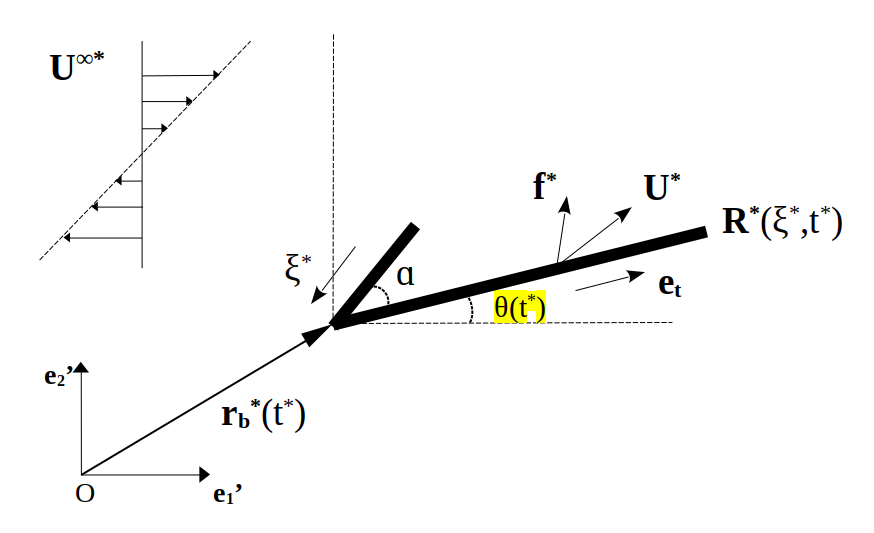
\includegraphics[width=0.8\textwidth]{plots/schematic/schematic_rigid_configuration_color2.png}
				\end{center}
				%	\setlength{\abovecaptionskip}{-0.5 cm}
			\end{figure}\vspace{0.3cm}
			\column{.5\textwidth}
			\small 	The local fluid traction on the fibre is given by: 
			\begin{equation*}
				\mathbf{f}^*=c_\perp\left(\mathbf{I}-\frac{1}{2}\mathbf{e}_t\mathbf{e}_t\right)\cdot(\mathbf{U}^{\infty*}-\mathbf{U}^*).
			\end{equation*}
		\end{columns}\vspace{-0.5cm}
		\begin{columns}
			\column{.55\textwidth}	
			\bi \small
			\item Net drag and net torque: 	\scriptsize
			\begin{equation*}
				\label{eqn:52}
				\textbf{F}^*=\int^\mathcal{L}_0 \textbf{f}^*\, \left|\frac{\partial\textbf{R}^*}{\partial\xi^*}\right|\,d\xi^*, 
			\end{equation*}
			\begin{equation*}
				\label{eqn:53}
				T^*_z=\textbf{e}_z\cdot\left\{\int^\mathcal{L}_0 \left[(\textbf{R}^*-\textbf{R}_c^*)\times \textbf{f}^*\,\right]\,\left|\frac{\partial\textbf{R}^*}{\partial\xi^*}\right|\,d\xi^*\right\},
			\end{equation*}\vspace{-0.3cm}
			\ei
			\column{.58\textwidth} \vspace{-0.1cm}
			\bi
			\item \small Find steady orientation:
			\scriptsize
			\begin{equation*}
				\left.\begin{aligned}
					\textbf{F}^*\,(\textbf{R}_0^*(\xi), \mathcal{V}, \mathcal{U}, \theta_{eq})=\textbf{0}\\
					T^*_z\,(\textbf{R}_0^*(\xi), \mathcal{V}, \mathcal{U}, \theta_{eq})=0\\
					\frac{d\theta(t^*)}{dt^*}=0
				\end{aligned}\right\}\Longrightarrow \colorbox{yellow}{$\theta_{eq},\mathcal{V}, \mathcal{U}$}.
			\end{equation*} 
			\ei
		\end{columns}
		\vspace{0.55cm}
		(Not quite the way Roggeveen $\&$ Stone did it...)
		%\selectfont \fontsize{10}{15}\selectfont
	\end{overlayarea}
\end{frame}

%%%%%%%%%%%%%%%%%%%%%%%%%%%%%%%%%%%%%%%%%%%%%%%%%%%%%%%%%%%%%%%%%%%%%%

\begin{frame}
	\frametitle{How to find non-rotating configurations?}
	\begin{overlayarea}{\textwidth}{\textheight}\vspace{-0.5cm}
Note: Fibres translate along parabolic trajectory:
		\begin{equation*}
			\bm{r}^*_b(t^*)=\left(\begin{aligned}
				&X(t^*) \\
				&Y(t^*)
			\end{aligned}\right)=\left(\begin{aligned}
				&\colorbox{yellow}{$\frac{1}{2}\mathcal{V}t^{*2}+\mathcal{U}t^*$}+X_{0} \\
				&\colorbox{yellow}{$\mathcal{V}t^*$}+Y_{0}
			\end{aligned}\right).
		\end{equation*}\vspace{-0.5cm}
		
		\foreach \index in {1,...,11} % 748}
        {\pgfmathsetmacro\picnumber{int(\index-1)}	
          \only<\index>{% FRAME: \index  \ \picnumber	
				\begin{center}
					\includegraphics[width=0.8\textwidth]{plots/plots_shape_rigid/rigid_plot_\picnumber.png}
				\end{center}
			}
		} 
	\end{overlayarea}
\end{frame}

%%%%%%%%%%%%%%%%%%%%%%%%%%%%%%%%%%%%%%%%%%%%%%%%%%%%%%%%%%%%%%%%%%%%%%



\begin{frame}
	\frametitle{Results: rotating and non-rotating solutions}
	\begin{overlayarea}{\textwidth}{\textheight}
		\vspace{-0.5cm}
		\begin{columns}
			\column{.6\textwidth}\vspace{0.2cm}
			$q-\alpha$ diagram:
			\bi
		\item \textbf{White} region: \textbf{rotation} (Jeffery orbits). 
		\item \textbf{Grey} region: \textbf{no rotation} 
		(for asymmetric shapes, small $\alpha$). 
		\ei 
			\column{.5\textwidth}
			\begin{figure}[htb]
				\begin{center}
					% specify width as 80% of the width of the text on the page
					% we can also specify a width in centimetres, e.g. [width=8cm]
					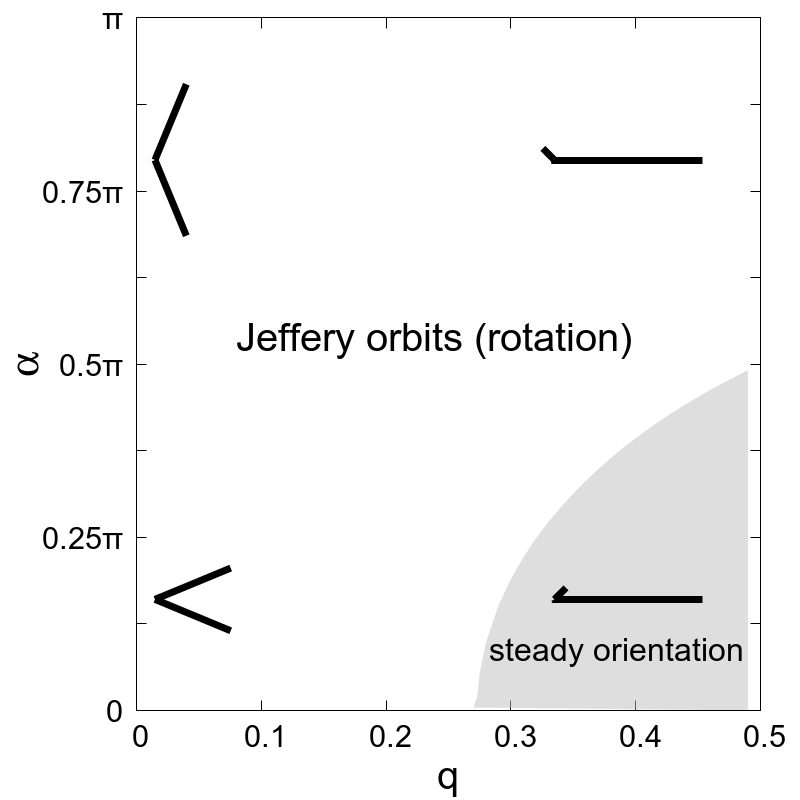
\includegraphics[width=0.85\textwidth]{plots/q_alpha_plot.png}
				\end{center}
				%	\setlength{\abovecaptionskip}{-0.5 cm}
			\end{figure}
		\end{columns}
		\vspace{0.5cm}
		\begin{columns}
			\column{.55\textwidth}
		\end{columns}
	\end{overlayarea}
\end{frame}

%%%%%%%%%%%%%%%%%%%%%%%%%%%%%%%%%%%%%%%%%%%%%%%%%%%%%%%%%%%%%%%%%%%%%%

\begin{frame}
	\frametitle{Results: rotating and non-rotating solutions}
	\begin{overlayarea}{\textwidth}{\textheight}
		\vspace{-0.5cm}
		\begin{columns}
			\column{.6\textwidth}\vspace{0.2cm}
			$q-\alpha$ diagram:
			\bi
			\item \textbf{White} region: \textbf{rotation} (Jeffery orbits). 
			\item \textbf{Grey} region: \textbf{no rotation}
			(for asymmetric shapes, small $\alpha$). 
			\ei 
			\column{.5\textwidth}
			\begin{figure}[htb]
				\begin{center}
					% specify width as 80% of the width of the text on the page
					% we can also specify a width in centimetres, e.g. [width=8cm]
					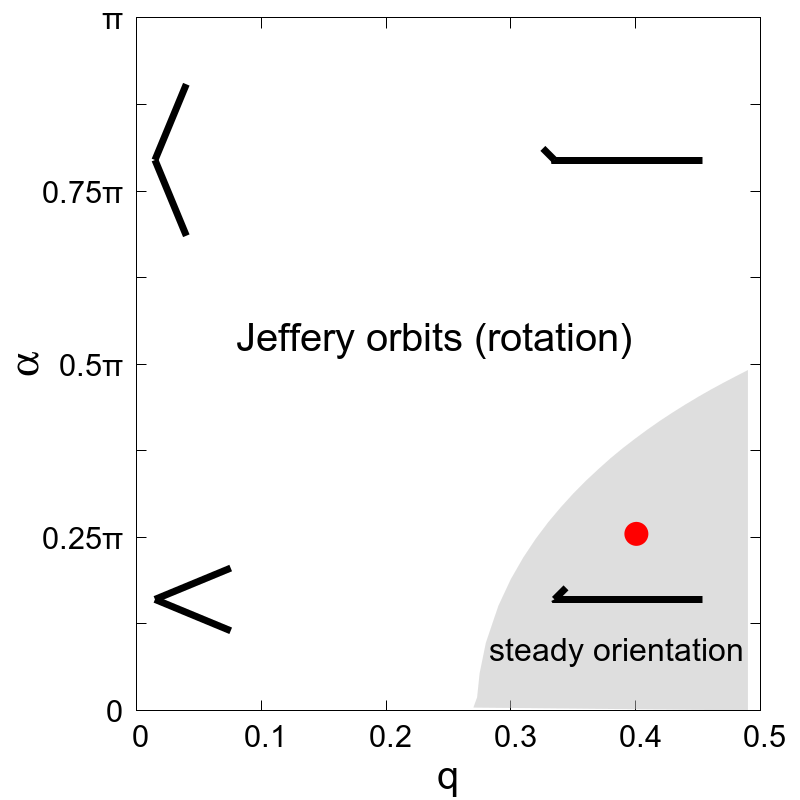
\includegraphics[width=0.85\textwidth]{plots/q_alpha_plot_with_point.png}
				\end{center}
				%	\setlength{\abovecaptionskip}{-0.5 cm}
			\end{figure}
		\end{columns}
		\vspace{0.3cm}
		\begin{columns}
			\column{.55\textwidth}\small
			For each $(q,\alpha)$ in steady regime:
			\bi
			\item Four equilibria.
			\item Two stable, two unstable. 
			\item Two stable (unstable) differ by $\pi$.
			\ei \vspace{0.5cm}
			\column{.6\textwidth}
			\vspace{-1cm}
			\begin{figure}[htb]
				\begin{center}
					% specify width as 80% of the width of the text on the page
					% we can also specify a width in centimetres, e.g. [width=8cm]
					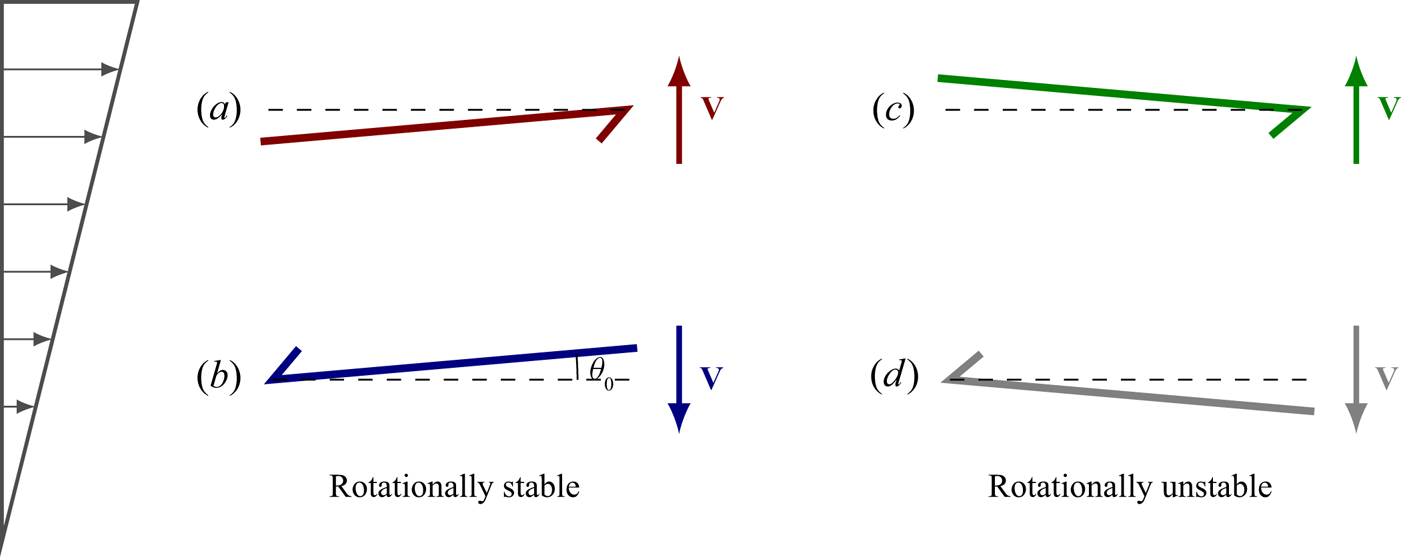
\includegraphics[width=1\textwidth]{plots/stone3.png}
				\end{center}
				%	\setlength{\abovecaptionskip}{-0.5 cm}
			\end{figure}
		\end{columns}
	\end{overlayarea}
\end{frame}

%%%%%%%%%%%%%%%%%%%%%%%%%%%%%%%%%%%%%%%%%%%%%%%%%%%%%%%%%%%%%%%%%%%%%%

\begin{frame}
	\frametitle{Results: rotating and non-rotating solutions}
	\begin{overlayarea}{\textwidth}{\textheight}
		
	Validation: 
		\begin{figure}
		\begin{minipage}{0.52\linewidth}
			\footnotesize 
			\centering			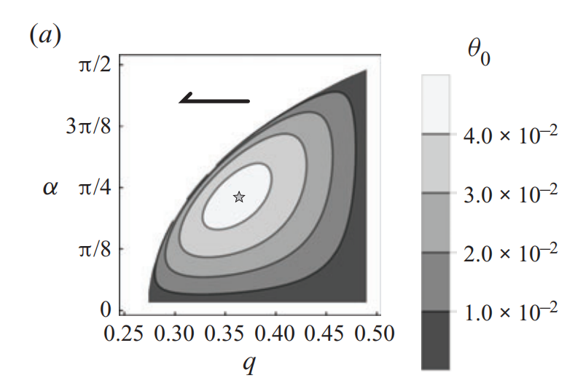
\includegraphics[width=\linewidth]{plots/plot10.png}
			\footnotesize Based on resistance matrix 
		\end{minipage}
		\begin{minipage}{0.45\linewidth}
			\centering
			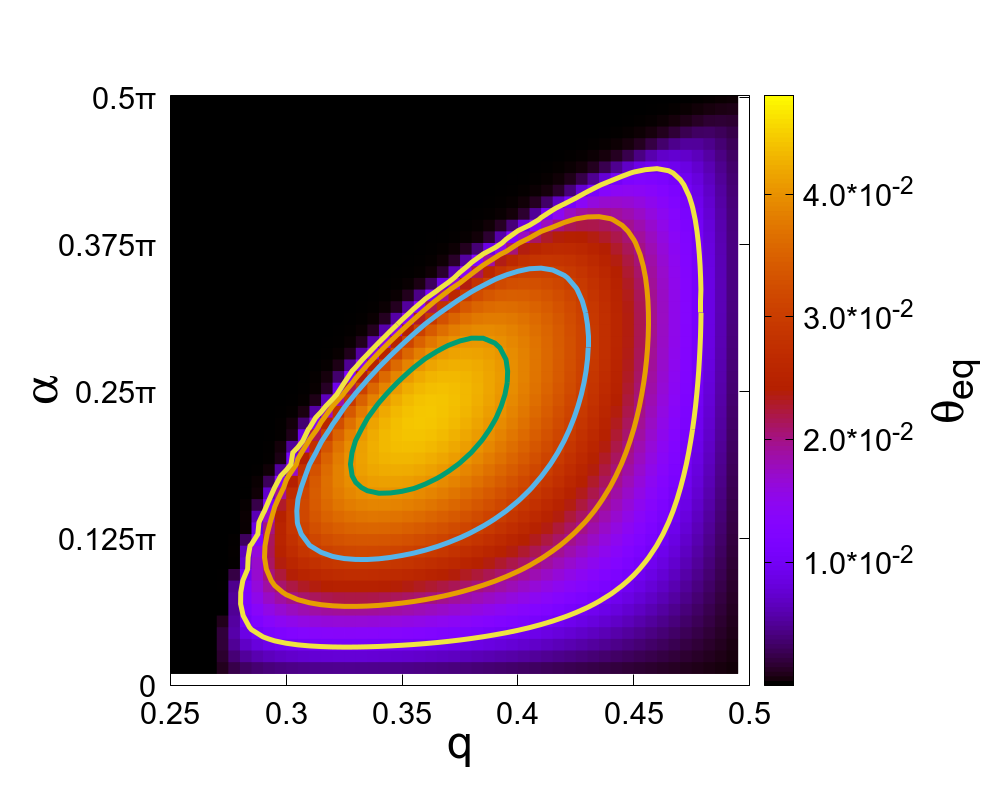
\includegraphics[width=\linewidth]{plots/numercial_straight_contour_theta_for_bamc.png}
			\footnotesize Based on balance of forces  
		\end{minipage}
	\end{figure}

\bi 
\item Our plot is identical to Roggeveen $\&$ Stone's result.
\ei 
	\end{overlayarea}
\end{frame}

%%%%%%%%%%%%%%%%%%%%%%%%%%%%%%%%%%%%%%%%%%%%%%%%%%%%%%%%%%%%%%%%%%%%%%

\begin{frame}
	\frametitle{The new bit: elasticity}
	\begin{overlayarea}{\textwidth}{\textheight}\vspace{1cm}
	\Large \bi
	\item Recall that in many applications, fibres are elastic.
	\vspace{1cm}
	\item \textbf{Aim of our work}: 
	
	Do steady solutions persist in the presence of elasticity (fluid-solid interaction)?
	\ei
	\end{overlayarea}
\end{frame}

%%%%%%%%%%%%%%%%%%%%%%%%%%%%%%%%%%%%%%%%%%%%%%%%%%%%%%%%%%%%%%%%%%%%%%

\begin{frame}
	\frametitle{The new bit: elasticity}
	\begin{overlayarea}{\textwidth}{\textheight}
\vspace{-0.5cm}
		\begin{columns}
		\column{.75\textwidth}	\vspace{-0.5cm}
		\begin{figure}[htb]
			\begin{center}
				% specify width as 80% of the width of the text on the page
				% we can also specify a width in centimetres, e.g. [width=8cm]
				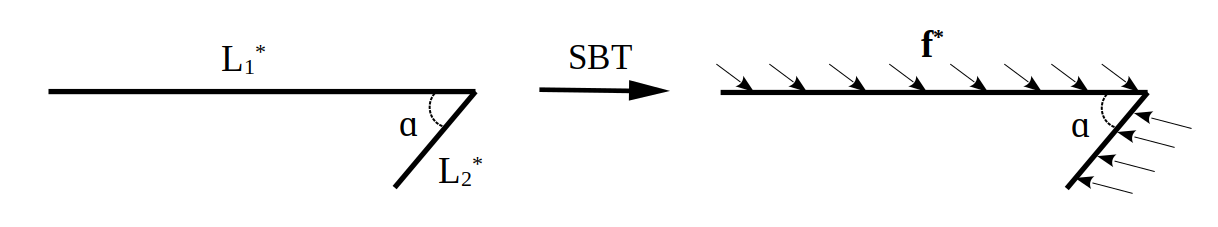
\includegraphics[width=1.05\textwidth]{plots/schematic/shape_to_traction.png}
			\end{center}
			%	\setlength{\abovecaptionskip}{-0.5 cm}
		\end{figure}
		\column{.4\textwidth}
		\bi 
		\item \small So far, SBT:
		
		 shape $\Longrightarrow$ traction $\mathbf{f}^*$.
		\ei
	\end{columns}
	\end{overlayarea}
\end{frame}

%%%%%%%%%%%%%%%%%%%%%%%%%%%%%%%%%%%%%%%%%%%%%%%%%%%%%%%%%%%%%%%%%%%%%%

\begin{frame}
	\frametitle{The new bit: elasticity}
	\begin{overlayarea}{\textwidth}{\textheight}
		\vspace{-0.5cm}
		\begin{columns}
			\column{.75\textwidth}	\vspace{-0.5cm}
			\begin{figure}[htb]
				\begin{center}
					% specify width as 80% of the width of the text on the page
					% we can also specify a width in centimetres, e.g. [width=8cm]
					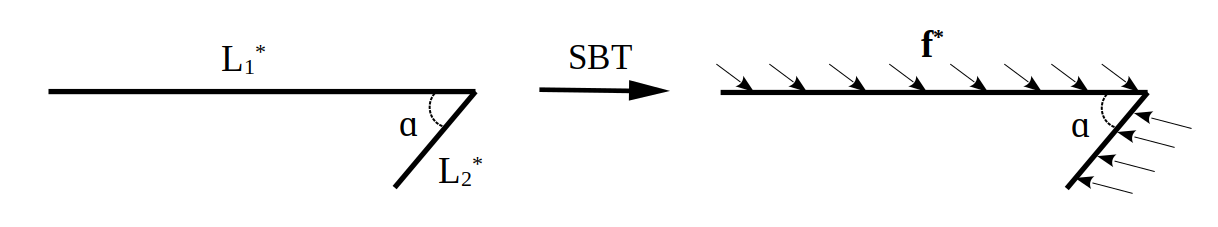
\includegraphics[width=1.05\textwidth]{plots/schematic/shape_to_traction.png}
				\end{center}
				%	\setlength{\abovecaptionskip}{-0.5 cm}
			\end{figure}
			\column{.4\textwidth}
			\bi 
			\item \small So far, SBT:
			
			shape $\Longrightarrow$ traction $\mathbf{f}^*$.
			\ei
		\end{columns}
		\begin{columns}
			\column{.75\textwidth}	\vspace{-1cm}
			\begin{figure}[htb]
				\begin{center}
					% specify width as 80% of the width of the text on the page
					% we can also specify a width in centimetres, e.g. [width=8cm]
					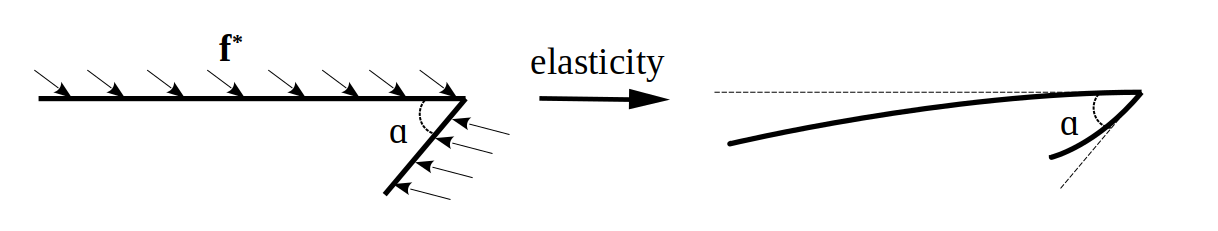
\includegraphics[width=1.05\textwidth]{plots/schematic/traction_to_shape.png}
				\end{center}
				%	\setlength{\abovecaptionskip}{-0.5 cm}
			\end{figure}
			\column{.4\textwidth}\vspace{-0.1cm}
			\bi 
			\item \small Now, elasticity:
			
			traction $\mathbf{f}^*$ $\Longrightarrow$ shape.
			\ei
		\end{columns}\vspace{0.2cm}
	\end{overlayarea}
\end{frame}

%%%%%%%%%%%%%%%%%%%%%%%%%%%%%%%%%%%%%%%%%%%%%%%%%%%%%%%%%%%%%%%%%%%%%%

\begin{frame}
	\frametitle{The new bit: elasticity}
	\begin{overlayarea}{\textwidth}{\textheight}
		\vspace{-0.5cm}
		\begin{columns}
			\column{.75\textwidth}	\vspace{-0.5cm}
			\begin{figure}[htb]
				\begin{center}
					% specify width as 80% of the width of the text on the page
					% we can also specify a width in centimetres, e.g. [width=8cm]
					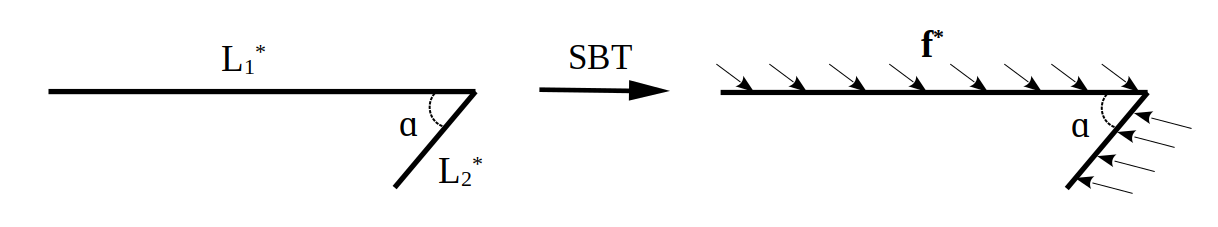
\includegraphics[width=1.05\textwidth]{plots/schematic/shape_to_traction.png}
				\end{center}
				%	\setlength{\abovecaptionskip}{-0.5 cm}
			\end{figure}
			\column{.4\textwidth}
			\bi 
			\item \small So far, SBT:
			
			shape $\Longrightarrow$ traction $\mathbf{f}^*$.
			\ei
		\end{columns}
		\begin{columns}
			\column{.75\textwidth}	\vspace{-1cm}
			\begin{figure}[htb]
				\begin{center}
					% specify width as 80% of the width of the text on the page
					% we can also specify a width in centimetres, e.g. [width=8cm]
					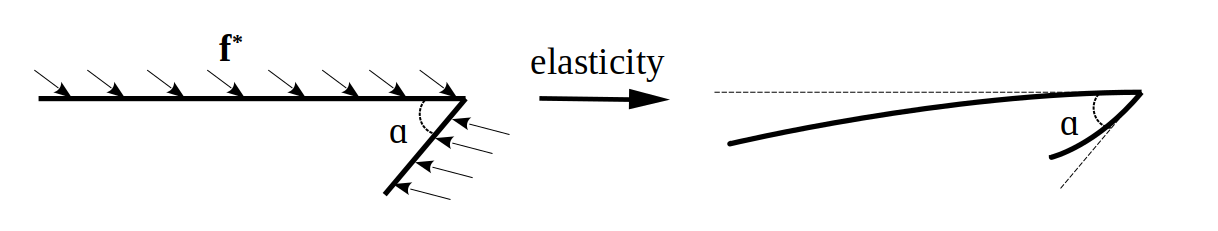
\includegraphics[width=1.05\textwidth]{plots/schematic/traction_to_shape.png}
				\end{center}
				%	\setlength{\abovecaptionskip}{-0.5 cm}
			\end{figure}
			\column{.4\textwidth}\vspace{-0.1cm}
			\bi 
			\item \small Now, elasticity:
			
			traction $\mathbf{f}^*$ $\Longrightarrow$ shape.
			\ei
		\end{columns}\vspace{0.2cm}
		\begin{columns}
			\column{.4\textwidth}	\vspace{-0.6cm} 
			\bi
			\item Fluid-solid interaction: 
			\ei
			\column{.65\textwidth} \vspace{-0.35cm}
			\begin{figure}[htb]
				\begin{center}
					% specify width as 80% of the width of the text on the page
					% we can also specify a width in centimetres, e.g. [width=8cm]
					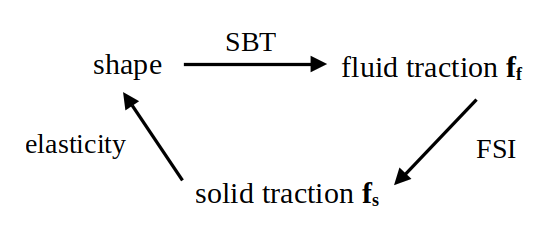
\includegraphics[width=0.9\textwidth]{plots/schematic/logic.png}
				\end{center}
				%	\setlength{\abovecaptionskip}{-0.5 cm}
			\end{figure}
		\end{columns}\vspace{0.1cm}
	\end{overlayarea}
\end{frame}

%%%%%%%%%%%%%%%%%%%%%%%%%%%%%%%%%%%%%%%%%%%%%%%%%%%%%%%%%%%%%%%%%%%%%%

\begin{frame}
	\frametitle{The new bit: elasticity}
	\begin{overlayarea}{\textwidth}{\textheight}
		\vspace{-0.5cm}
		\begin{columns}
			\column{.75\textwidth}	\vspace{-0.5cm}
			\begin{figure}[htb]
				\begin{center}
					% specify width as 80% of the width of the text on the page
					% we can also specify a width in centimetres, e.g. [width=8cm]
					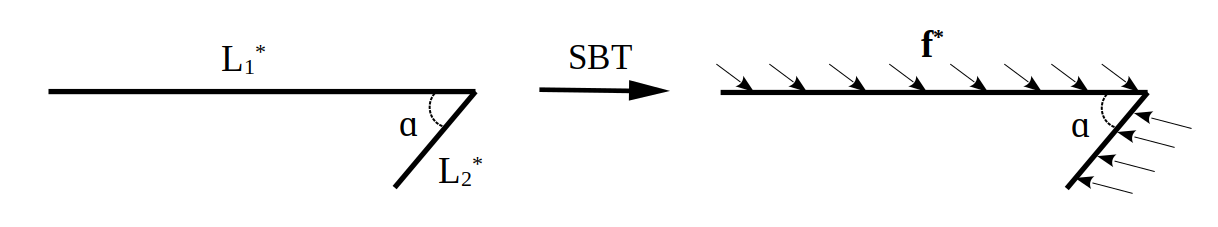
\includegraphics[width=1.05\textwidth]{plots/schematic/shape_to_traction.png}
				\end{center}
				%	\setlength{\abovecaptionskip}{-0.5 cm}
			\end{figure}
			\column{.4\textwidth}
			\bi 
			\item \small So far, SBT:
			
			shape $\Longrightarrow$ traction $\mathbf{f}^*$.
			\ei
		\end{columns}
		\begin{columns}
			\column{.75\textwidth}	\vspace{-1cm}
			\begin{figure}[htb]
				\begin{center}
					% specify width as 80% of the width of the text on the page
					% we can also specify a width in centimetres, e.g. [width=8cm]
					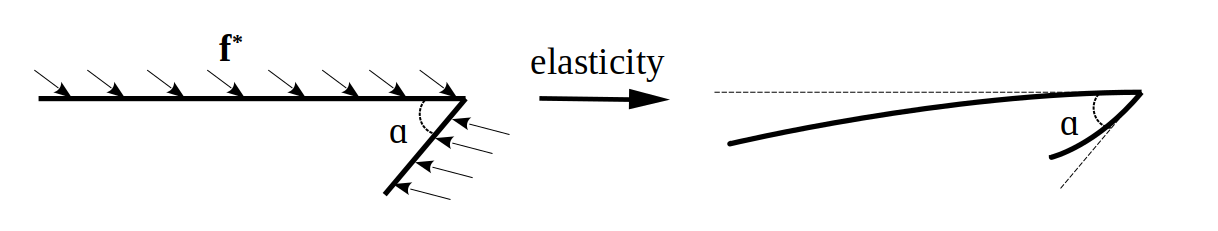
\includegraphics[width=1.05\textwidth]{plots/schematic/traction_to_shape.png}
				\end{center}
				%	\setlength{\abovecaptionskip}{-0.5 cm}
			\end{figure}
			\column{.4\textwidth}\vspace{-0.1cm}
			\bi 
			\item \small Now, elasticity:
			
			traction $\mathbf{f}^*$ $\Longrightarrow$ shape.
			\ei
		\end{columns}\vspace{0.2cm}
		\begin{columns}
			\column{.4\textwidth}	\vspace{-0.6cm} 
			\bi
			\item Fluid-solid interaction: 
			\ei
			\column{.65\textwidth} \vspace{-0.35cm}
			\begin{figure}[htb]
				\begin{center}
					% specify width as 80% of the width of the text on the page
					% we can also specify a width in centimetres, e.g. [width=8cm]
					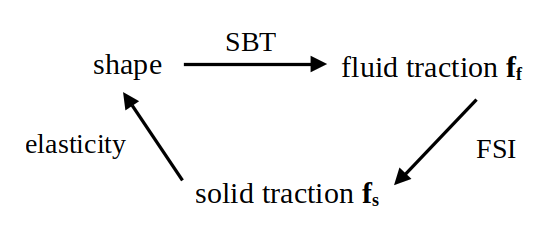
\includegraphics[width=0.9\textwidth]{plots/schematic/logic.png}
				\end{center}
				%	\setlength{\abovecaptionskip}{-0.5 cm}
			\end{figure}
		\end{columns}\vspace{0.1cm}
	...but actually solved "monolithically" (Newton's method acting on fully coupled equations).
	\end{overlayarea}
\end{frame}

%%%%%%%%%%%%%%%%%%%%%%%%%%%%%%%%%%%%%%%%%%%%%%%%%%%%%%%%%%%%%%%%%%%%%%


\begin{frame}
	\frametitle{The new bit: elasticity}
	\begin{overlayarea}{\textwidth}{\textheight}
		\vspace{-0.5cm}
       \small Kirchhoff-Love beam theory (Our library: \texttt{oomph-lib}):
		\vspace{-0.1cm} 
		\begin{equation*}
			\int^{\mathcal{L}}_0 \left[\mathscr{E}\,\gamma\, \delta\gamma+\mathscr{B}\,\kappa^*\,\delta\kappa^*-\sqrt{\frac{A}{a}}\bm{f}^*\cdot \delta\bm{R}^*\right]\sqrt{a}\,d\xi^*=0,
		\end{equation*}
		\begin{columns}
		\column{.6\textwidth}
	where 
	\bi
	\item $\mathscr{E}=\frac{Eh^*}{1-\nu^2}$ is the extensional stiffness,
	\item $\mathscr{B}=\frac{Eh^{*3}}{12(1-\nu^2)}$ is the bending stiffness,
	\item $\gamma$ is the strain tensor,
	\item $\kappa^*$ is the bending tensor,
	\item $A,a$ are the metric tensors of the beam's centreline, in the deformed and undeformed configurations. 
	\item $\xi^*$ is the Lagrangian coordinate.
	\ei
	\column{.55\textwidth}\vspace{-0.8cm}
	\begin{figure}[htb]
		\begin{center}
			% specify width as 80% of the width of the text on the page
			% we can also specify a width in centimetres, e.g. [width=8cm]
			
\includegraphics[width=0.4\textwidth]{plots/logo.png}
		\end{center}
		%	\setlength{\abovecaptionskip}{-0.5 cm}
	\end{figure}\vspace{-0.4cm}
\footnotesize \centering https://www.oomph-lib.org \small
	\begin{figure}[htb]
		\begin{center}
			% specify width as 80% of the width of the text on the page
			% we can also specify a width in centimetres, e.g. [width=8cm]
			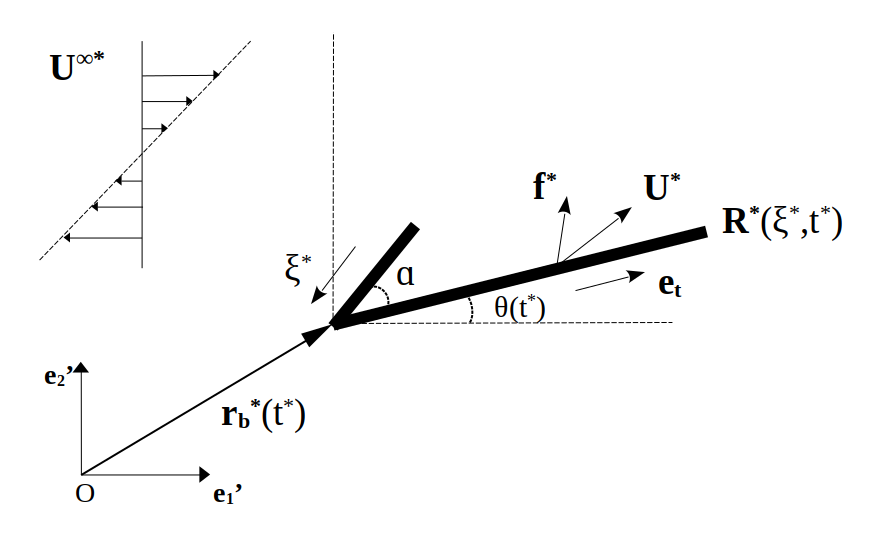
\includegraphics[width=1\textwidth]{plots/schematic/schematic_rigid_configuration_color0_old.png}
		\end{center}
		%	\setlength{\abovecaptionskip}{-0.5 cm}
	\end{figure}

\end{columns}
	\end{overlayarea}
\end{frame}

%%%%%%%%%%%%%%%%%%%%%%%%%%%%%%%%%%%%%%%%%%%%%%%%%%%%%%%%%%%%%%%%%%%%%%



\begin{frame}
	\frametitle{Fluid-solid interaction/Nondimensionalization}
	\begin{overlayarea}{\textwidth}{\textheight}\vspace{-0.5cm}
	\small Nondimensionalise the equations on appropriate scales:
	\bi 
	\item Slender body theory (scale on viscous stresses):\vspace{-0.1cm}
	\begin{equation*}
		\mathbf{f}^*=c_\perp\,\mathcal{L}\,\dot{\gamma}\,\mathbf{f}_{f}.
	\end{equation*}
    \item Kirchhoff-Love beam theory (scale on bending stiffness):\vspace{-0.1cm}
    \begin{equation*}
    	\mathbf{f}^*=\frac{\mathscr{B}}{\mathcal{L}^3}\,\mathbf{f}_{s}.
    \end{equation*}
    \ei 
   	\vspace{-0.2cm} FSI parameter: 
   	\begin{equation*}
   		\label{eqn:38}
   		\mathcal{I}=\frac{c_\perp\,\mathcal{L}^4\,\dot{\gamma}}{\mathscr{B}}=\frac{\text{"fluid stress"}}{\text{"bending stiffness"}}.
   	\end{equation*}
   \vspace{-0.3cm}\small \bi
   \item Traction on beam:
	\begin{equation*}
		\textbf{f}_{s}=\mathcal{I}\,\textbf{f}_{f},
	\end{equation*}
			 \item $\mathcal{I}=0$: rigid; \quad $\mathcal{I}>0$: elastic.
			 \ei
	\end{overlayarea}
\end{frame}



%%%%%%%%%%%%%%%%%%%%%%%%%%%%%%%%%%%%%%%%%%%%%%%%%%%%%%%%%%%%%%%%%%%%%%



\begin{frame}
	\frametitle{How to find steady orientation (FSI)?}
	\begin{overlayarea}{\textwidth}{\textheight}
		\vspace{-0.6cm}	
			\begin{figure}[htb]
			\begin{center}
				% specify width as 80% of the width of the text on the page
				% we can also specify a width in centimetres, e.g. [width=8cm]
				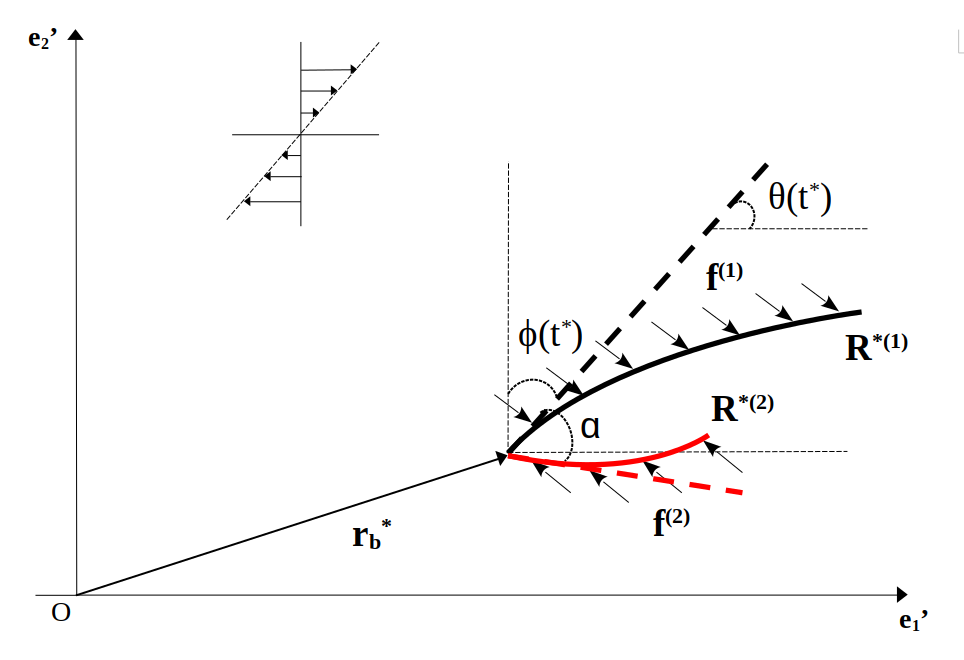
\includegraphics[width=0.65\textwidth]{plots/schematic/traction_on_particle.png}
			\end{center}
			%	\setlength{\abovecaptionskip}{-0.5 cm}
		\end{figure}	
      Equations: 
		$\quad \quad\quad
	\left.	\begin{aligned}
			\colorbox{yellow}{\text{beam equation}}\\
			\colorbox{green}{\text{drag-free}}\\
			\colorbox{green}{\text{torque-free}}\\
			\colorbox{green}{\text{no rotation}}
		\end{aligned}\right\}\Longrightarrow \colorbox{green}{$\theta_{eq}, \mathcal{V}, \mathcal{U}$},$\colorbox{yellow}{deformation}.	
	\end{overlayarea}
\end{frame}

%%%%%%%%%%%%%%%%%%%%%%%%%%%%%%%%%%%%%%%%%%%%%%%%%%%%%%%%%%%%%%%%%%%%%%

\begin{frame}
	\frametitle{\mbox{}}
	\begin{overlayarea}{\textwidth}{\textheight}
		\vspace{2.5cm}	
	\Huge \centering Results (with FSI).
	\end{overlayarea}
\end{frame}

%%%%%%%%%%%%%%%%%%%%%%%%%%%%%%%%%%%%%%%%%%%%%%%%%%%%%%%%%%%%%%%%%%%%%%


\begin{frame}
	\frametitle{Results: effect of FSI}
	% Define an overlay area that covers the full slide
	\begin{overlayarea}{\textwidth}{\textheight}
		\vspace{-0.3cm}  % Reduce space above image		
		\begin{figure}[htb]
		\begin{center}
			% specify width as 80% of the width of the text on the page
			% we can also specify a width in centimetres, e.g. [width=8cm]
			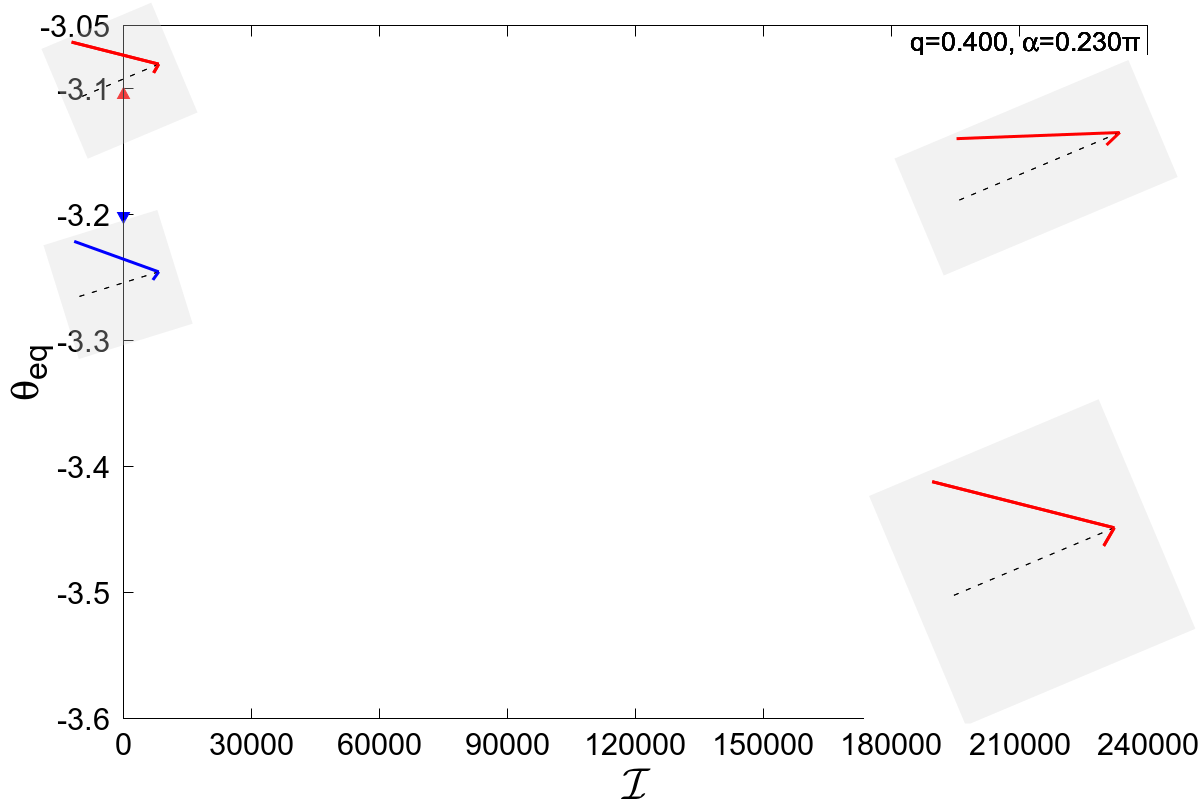
\includegraphics[width=0.9\textwidth]{plots/RESLT_q_0.40_alpha_0.230pi_plot_step_refine2_new_recale_FSI_slides/combine_elastic_beam_I_theta_q_0.40_alpha_0.230pi_initial_-4.80_refine2_new_not_log_0.png}
		\end{center}
		%	\setlength{\abovecaptionskip}{-0.5 cm}
	\end{figure}	
		\vspace{-0.3cm}  % Reduce space below the image
		
		% Bullet-point list under the image
		\begin{itemize}
			\item $\mathcal{I}=0$ (rigid), two known solutions: one stable, one unstable.
			\item Note non-unit aspect ratio in shape plots.
		\end{itemize}
			\begin{tikzpicture}[remember picture, overlay]
			\node[anchor=north west, text=black, font=\small\bfseries]
			at ([xshift=0.15cm,yshift=-1.9cm]current page.north west) {stable};
	    	\end{tikzpicture}
			\begin{tikzpicture}[remember picture, overlay]
				\node[anchor=north west, text=black, font=\small\bfseries]
				at ([xshift=0.15cm,yshift=-2.9cm]current page.north west) {unstable};
		\end{tikzpicture}
\begin{tikzpicture}[remember picture, overlay]
	\node[anchor=north west, text=black, font=\small\bfseries, rotate=23]
	at ([xshift=9cm,yshift=-3.6cm]current page.north west) {1:1 aspect ratio};
\end{tikzpicture}
\begin{tikzpicture}[remember picture, overlay]
	\node[anchor=north west, text=black, font=\small\bfseries, rotate=23]
	at ([xshift=9cm,yshift=-6.9cm]current page.north west) {stretched vertically};
\end{tikzpicture}
	\end{overlayarea}
\end{frame}


%%%%%%%%%%%%%%%%%%%%%%%%%%%%%%%%%%%%%%%%%%%%%%%%%%%%%%%%%%%%%%%%%%%%%%

\begin{frame}
	\frametitle{Results: effect of FSI}
	% Define an overlay area that covers the full slide
	\begin{overlayarea}{\textwidth}{\textheight}
		\vspace{-0.3cm}  % Reduce space above image		
		\begin{figure}[htb]
			\begin{center}
				% specify width as 80% of the width of the text on the page
				% we can also specify a width in centimetres, e.g. [width=8cm]
				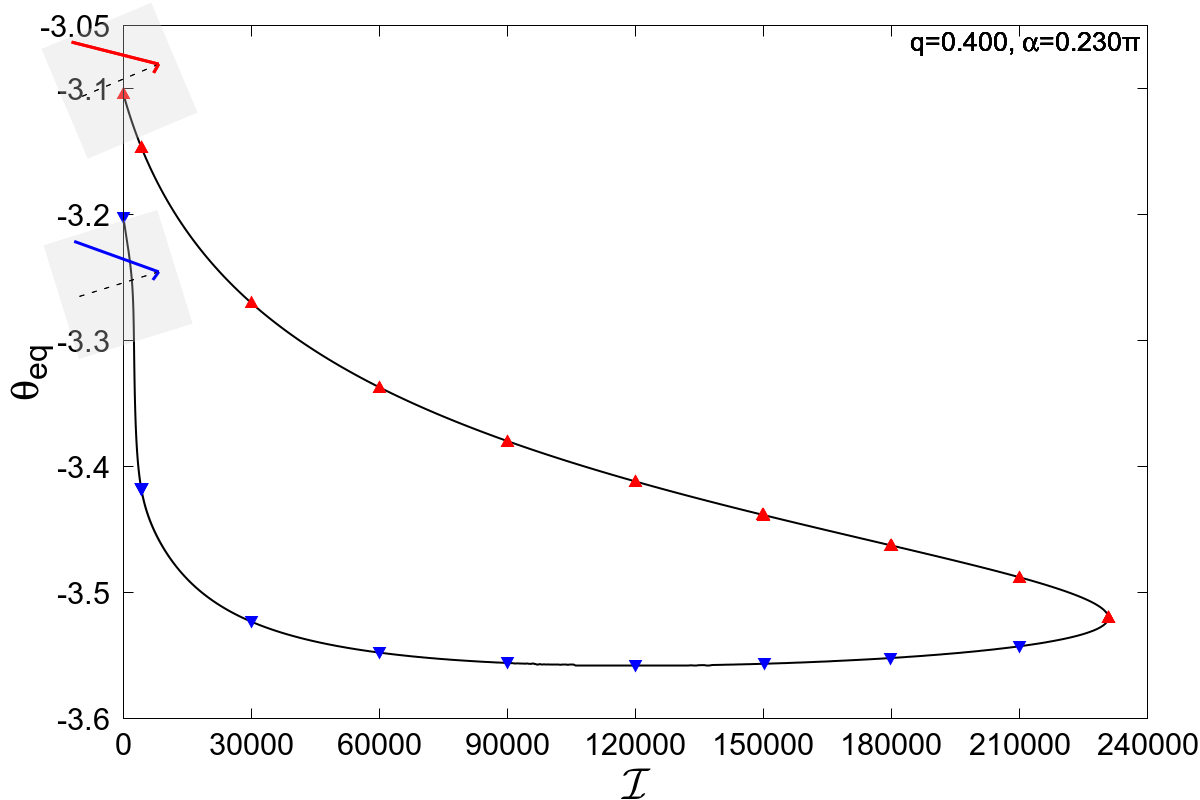
\includegraphics[width=0.9\textwidth]{plots/RESLT_q_0.40_alpha_0.230pi_plot_step_refine2_new_recale_FSI_slides/combine_elastic_beam_I_theta_q_0.40_alpha_0.230pi_initial_-4.80_refine2_new_not_log_1.png}
			\end{center}
			%	\setlength{\abovecaptionskip}{-0.5 cm}
		\end{figure}	
		\vspace{-0.3cm}  % Reduce space below the image
		
		% Bullet-point list under the image
		\bi\small
\item Two solution branches emerge from $\mathcal{I}=0$.
\item Steady solutions exist up to $\mathcal{I}_{max}(q,\alpha)$ at which the two branches meet in a limit point.
\ei
		\begin{tikzpicture}[remember picture, overlay]
			\node[anchor=north west, text=black, font=\small\bfseries]
			at ([xshift=0.15cm,yshift=-1.9cm]current page.north west) {stable};
		\end{tikzpicture}
		\begin{tikzpicture}[remember picture, overlay]
			\node[anchor=north west, text=black, font=\small\bfseries]
			at ([xshift=0.15cm,yshift=-2.9cm]current page.north west) {unstable};
		\end{tikzpicture}
	\end{overlayarea}
\end{frame}


%%%%%%%%%%%%%%%%%%%%%%%%%%%%%%%%%%%%%%%%%%%%%%%%%%%%%%%%%%%%%%%%%%%%%%


\begin{frame}
	\frametitle{Results: effect of FSI}
	% Define an overlay area that covers the full slide
	\begin{overlayarea}{\textwidth}{\textheight}
		\vspace{-0.3cm}  % Reduce space above image		
		\begin{figure}[htb]
			\begin{center}
				% specify width as 80% of the width of the text on the page
				% we can also specify a width in centimetres, e.g. [width=8cm]
				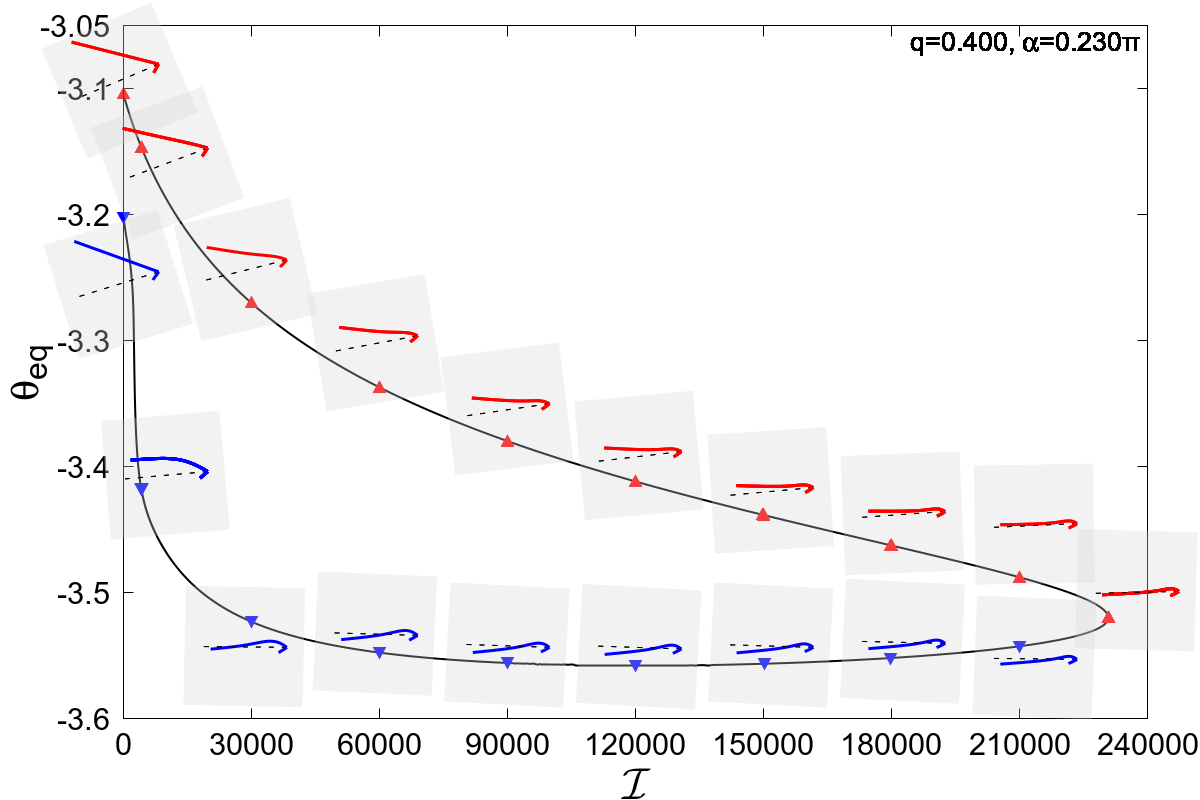
\includegraphics[width=0.9\textwidth]{plots/RESLT_q_0.40_alpha_0.230pi_plot_step_refine2_new_recale_FSI_slides/combine_elastic_beam_I_theta_q_0.40_alpha_0.230pi_initial_-4.80_refine2_new_not_log_18.png}
			\end{center}
			%	\setlength{\abovecaptionskip}{-0.5 cm}
		\end{figure}	
		\vspace{-0.3cm}  % Reduce space below the image
		\bi
		\item Fibre deforms modestly.
		\ei
		% Bullet-point list under the image
		\begin{tikzpicture}[remember picture, overlay]
			\node[anchor=north west, text=black, font=\small\bfseries]
			at ([xshift=0.15cm,yshift=-1.9cm]current page.north west) {stable};
		\end{tikzpicture}
		\begin{tikzpicture}[remember picture, overlay]
			\node[anchor=north west, text=black, font=\small\bfseries]
			at ([xshift=0.15cm,yshift=-2.9cm]current page.north west) {unstable};
		\end{tikzpicture}
	\end{overlayarea}
\end{frame}


%%%%%%%%%%%%%%%%%%%%%%%%%%%%%%%%%%%%%%%%%%%%%%%%%%%%%%%%%%%%%%%%%%%%%%


\begin{frame}
	\frametitle{Results: change in $\alpha$}
	% Define an overlay area that covers the full slide
	\begin{overlayarea}{\textwidth}{\textheight}
		\vspace{-0.3cm}  % Reduce space above image		
		\begin{figure}[htb]
			\begin{center}
				% specify width as 80% of the width of the text on the page
				% we can also specify a width in centimetres, e.g. [width=8cm]
				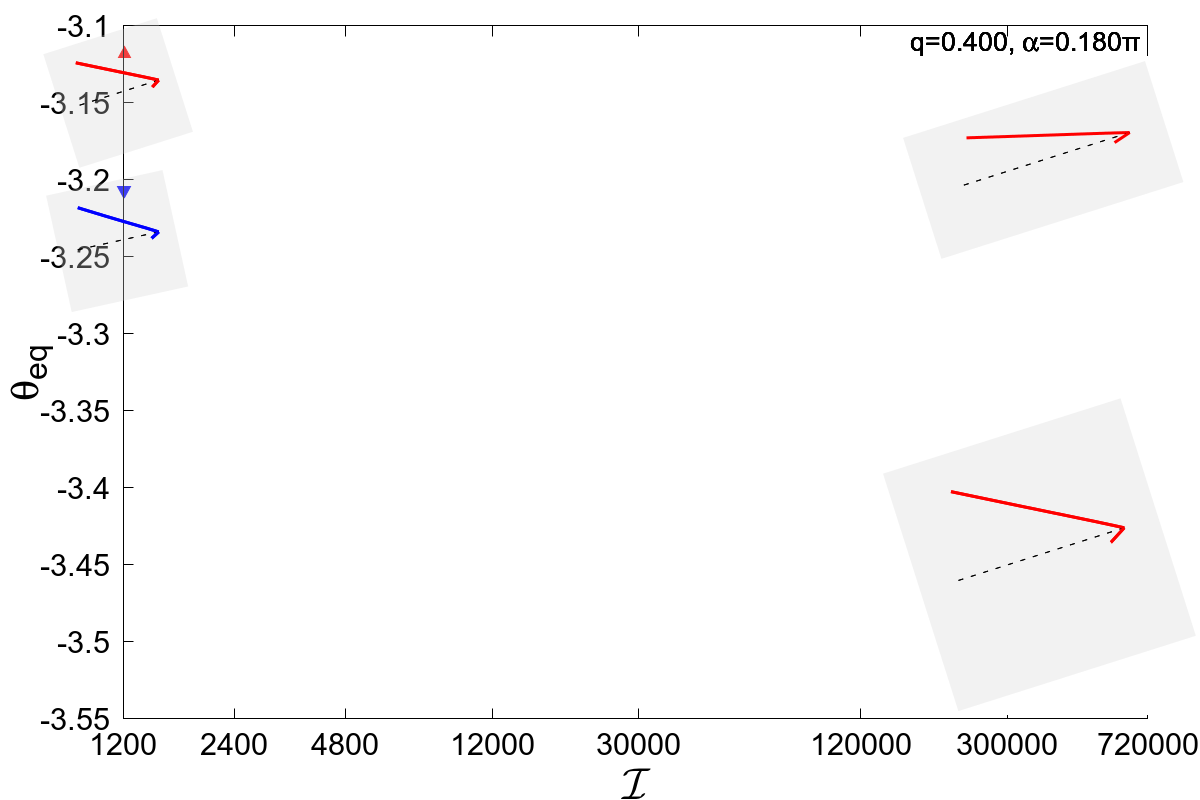
\includegraphics[width=0.9\textwidth]{plots/RESLT_q_0.400_alpha_0.180pi_plot_initial_step_refine2_new_recale_FSI_slides/initial_combine_elastic_beam_I_theta_q_0.400_alpha_0.180pi_initial_-4.80_refine2_new_0.png}
			\end{center}
			%	\setlength{\abovecaptionskip}{-0.5 cm}
		\end{figure}	
		\vspace{-0.3cm}  % Reduce space below the image
		
		% Bullet-point list under the image
			\bi
	\item Smaller $\alpha$.
	\item Again start with two known rigid solutions.
	\ei
		\begin{tikzpicture}[remember picture, overlay]
			\node[anchor=north west, text=black, font=\small\bfseries]
			at ([xshift=0.15cm,yshift=-1.5cm]current page.north west) {stable};
		\end{tikzpicture}
		\begin{tikzpicture}[remember picture, overlay]
			\node[anchor=north west, text=black, font=\small\bfseries]
			at ([xshift=0.15cm,yshift=-2.6cm]current page.north west) {unstable};
		\end{tikzpicture}
		\begin{tikzpicture}[remember picture, overlay]
			\node[anchor=north west, text=black, font=\small\bfseries, rotate=18]
			at ([xshift=9cm,yshift=-3.45cm]current page.north west) {1:1 aspect ratio};
		\end{tikzpicture}
		\begin{tikzpicture}[remember picture, overlay]
			\node[anchor=north west, text=black, font=\small\bfseries, rotate=18]
			at ([xshift=9cm,yshift=-6.8cm]current page.north west) {stretched vertically};
		\end{tikzpicture}
	\end{overlayarea}
\end{frame}


%%%%%%%%%%%%%%%%%%%%%%%%%%%%%%%%%%%%%%%%%%%%%%%%%%%%%%%%%%%%%%%%%%%%%%


\begin{frame}
	\frametitle{Results: change in $\alpha$}
	% Define an overlay area that covers the full slide
	\begin{overlayarea}{\textwidth}{\textheight}
		\vspace{-0.3cm}  % Reduce space above image		
		\begin{figure}[htb]
			\begin{center}
				% specify width as 80% of the width of the text on the page
				% we can also specify a width in centimetres, e.g. [width=8cm]
				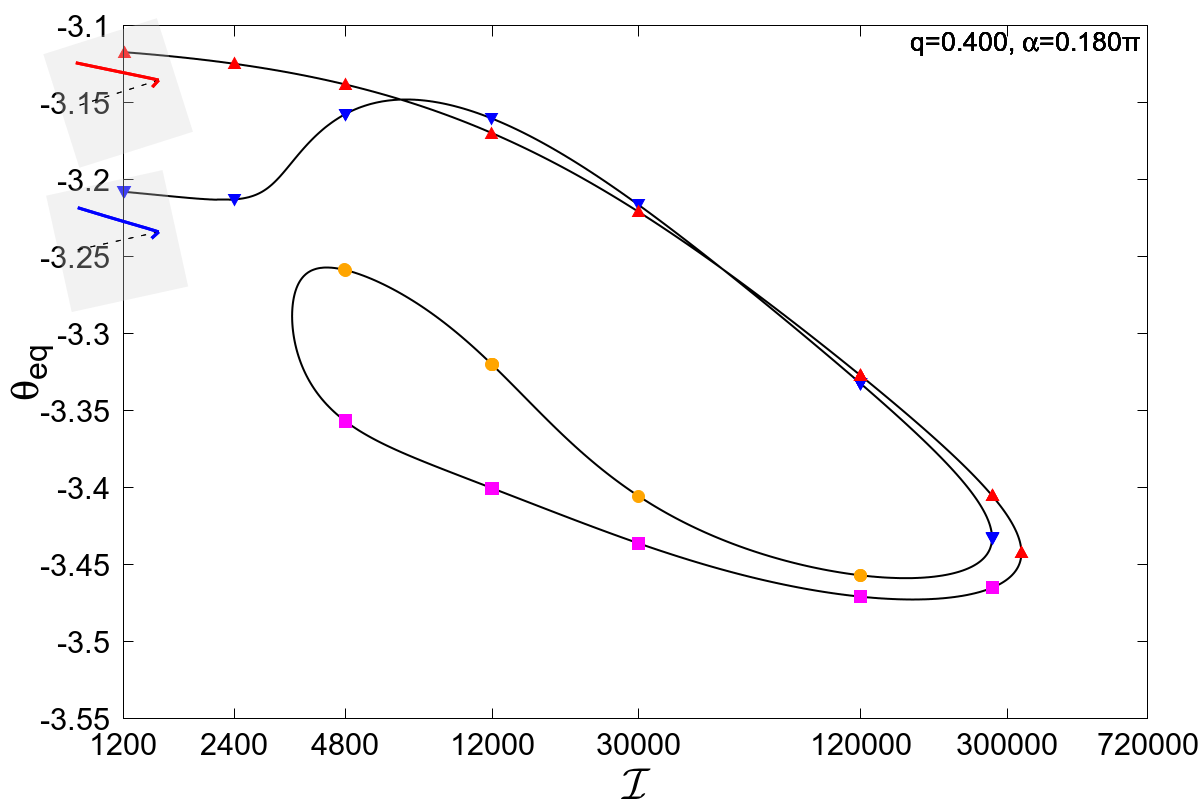
\includegraphics[width=0.9\textwidth]{plots/RESLT_q_0.400_alpha_0.180pi_plot_initial_step_refine2_new_recale_FSI_slides/initial_combine_elastic_beam_I_theta_q_0.400_alpha_0.180pi_initial_-4.80_refine2_new_1.png}
			\end{center}
			%	\setlength{\abovecaptionskip}{-0.5 cm}
		\end{figure}	
		\vspace{-0.3cm}  % Reduce space below the image
		
		% Bullet-point list under the image
		\bi
		\item This looks quite different!
		\ei
		\begin{tikzpicture}[remember picture, overlay]
			\node[anchor=north west, text=black, font=\small\bfseries]
			at ([xshift=0.15cm,yshift=-1.5cm]current page.north west) {stable};
		\end{tikzpicture}
		\begin{tikzpicture}[remember picture, overlay]
			\node[anchor=north west, text=black, font=\small\bfseries]
			at ([xshift=0.15cm,yshift=-2.6cm]current page.north west) {unstable};
		\end{tikzpicture}
	\end{overlayarea}
\end{frame}


%%%%%%%%%%%%%%%%%%%%%%%%%%%%%%%%%%%%%%%%%%%%%%%%%%%%%%%%%%%%%%%%%%%%%%

\begin{frame}
	\frametitle{Results: change in $\alpha$}
	% Define an overlay area that covers the full slide
	\begin{overlayarea}{\textwidth}{\textheight}
		\vspace{-0.3cm}  % Reduce space above image		
		\begin{figure}[htb]
			\begin{center}
				% specify width as 80% of the width of the text on the page
				% we can also specify a width in centimetres, e.g. [width=8cm]
				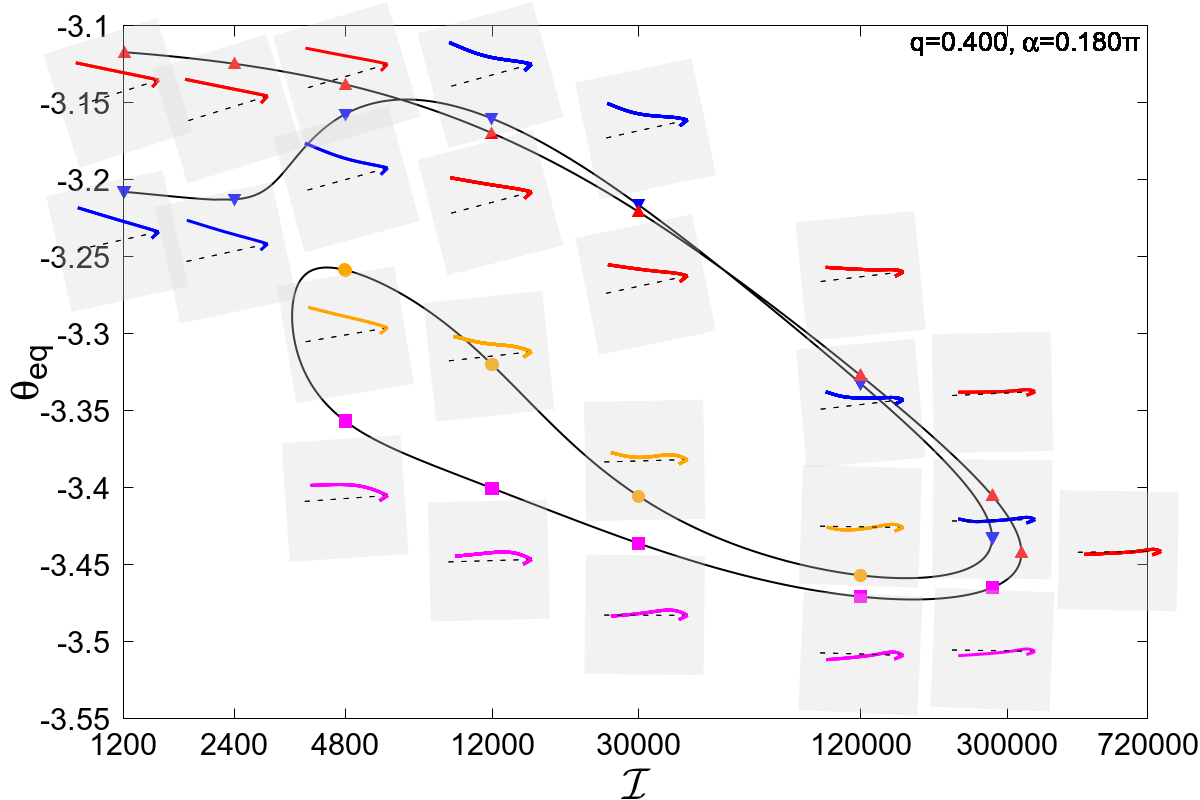
\includegraphics[width=0.9\textwidth]{plots/RESLT_q_0.400_alpha_0.180pi_plot_initial_step_refine2_new_recale_FSI_slides/initial_combine_elastic_beam_I_theta_q_0.400_alpha_0.180pi_initial_-4.80_refine2_new_5.png}
			\end{center}
			%	\setlength{\abovecaptionskip}{-0.5 cm}
		\end{figure}	
		\vspace{-0.3cm}  % Reduce space below the image
		\bi
		\item Different modes of deformation on different solution branches.
		\ei 
		% Bullet-point list under the image
		\begin{tikzpicture}[remember picture, overlay]
			\node[anchor=north west, text=black, font=\small\bfseries]
			at ([xshift=0.15cm,yshift=-1.5cm]current page.north west) {stable};
		\end{tikzpicture}
		\begin{tikzpicture}[remember picture, overlay]
			\node[anchor=north west, text=black, font=\small\bfseries]
			at ([xshift=0.15cm,yshift=-2.6cm]current page.north west) {unstable};
		\end{tikzpicture}
	\end{overlayarea}
\end{frame}


%%%%%%%%%%%%%%%%%%%%%%%%%%%%%%%%%%%%%%%%%%%%%%%%%%%%%%%%%%%%%%%%%%%%%%

\begin{frame}
	\frametitle{How does this happen?}
	\begin{overlayarea}{\textwidth}{\textheight}\vspace{-0.5cm}
		\foreach \index in {1,...,3} % 210}
	{\pgfmathsetmacro\picnumber{int(\index-1)}	
		\only<\index>{% FRAME: \index  \ \picnumber	
			\begin{center}	
				\includegraphics<\index>[width=0.65\textwidth]{plots/RESLT_animation_varying_alpha_q_0.400_step_rescale_FSI_slides/elastic_beam_I_theta_q_0.400_alpha_\picnumber.png}	
			\end{center}              	
			%\includegraphics<\index>[width=2\textwidth]{images/warped_disk/fe_soln/resized/frame\picnumber.png}}
		\vspace{-0.4cm}
		\bi\small
		\item Evaluation of diagram with $\alpha$.
		\ei	
	}
	%\scalebox{1.0}{\import{\PaperImagePath}{trajectories_Rc=0.5_red_karaoke/frame1.tex}}	
}
\end{overlayarea}
\end{frame}

%%%%%%%%%%%%%%%%%%%%%%%%%%%%%%%%%%%%%%%%%%%%%%%%%%%%%%%%%%%%%%%%%%%%%%


\begin{frame}
	\frametitle{How does this happen?}
	\begin{overlayarea}{\textwidth}{\textheight}\vspace{-0.5cm}
	\foreach \index in {1,...,3} % 210}
{\pgfmathsetmacro\picnumber{int(\index+2)}	
	\only<\index>{% FRAME: \index  \ \picnumber	
		\begin{center}	
			\includegraphics<\index>[width=0.65\textwidth]{plots/RESLT_animation_varying_alpha_q_0.400_step_rescale_FSI_slides/elastic_beam_I_theta_q_0.400_alpha_\picnumber.png}	
		\end{center}              	
		%\includegraphics<\index>[width=2\textwidth]{images/warped_disk/fe_soln/resized/frame\picnumber.png}}
	\vspace{-0.4cm}
	\bi\small
	\item Connection with initially disconnected loop (blue).
	\ei	
}
%\scalebox{1.0}{\import{\PaperImagePath}{trajectories_Rc=0.5_red_karaoke/frame1.tex}}	
}
\end{overlayarea}
\end{frame}

%%%%%%%%%%%%%%%%%%%%%%%%%%%%%%%%%%%%%%%%%%%%%%%%%%%%%%%%%%%%%%%%%%%%%%


\begin{frame}
	\frametitle{How does this happen?}
	% Define an overlay area that covers the full slide
	\begin{overlayarea}{\textwidth}{\textheight}
		\vspace{-0.3cm}  % Reduce space above image		
		\begin{figure}[htb]
			\begin{center}
				% specify width as 80% of the width of the text on the page
				% we can also specify a width in centimetres, e.g. [width=8cm]
				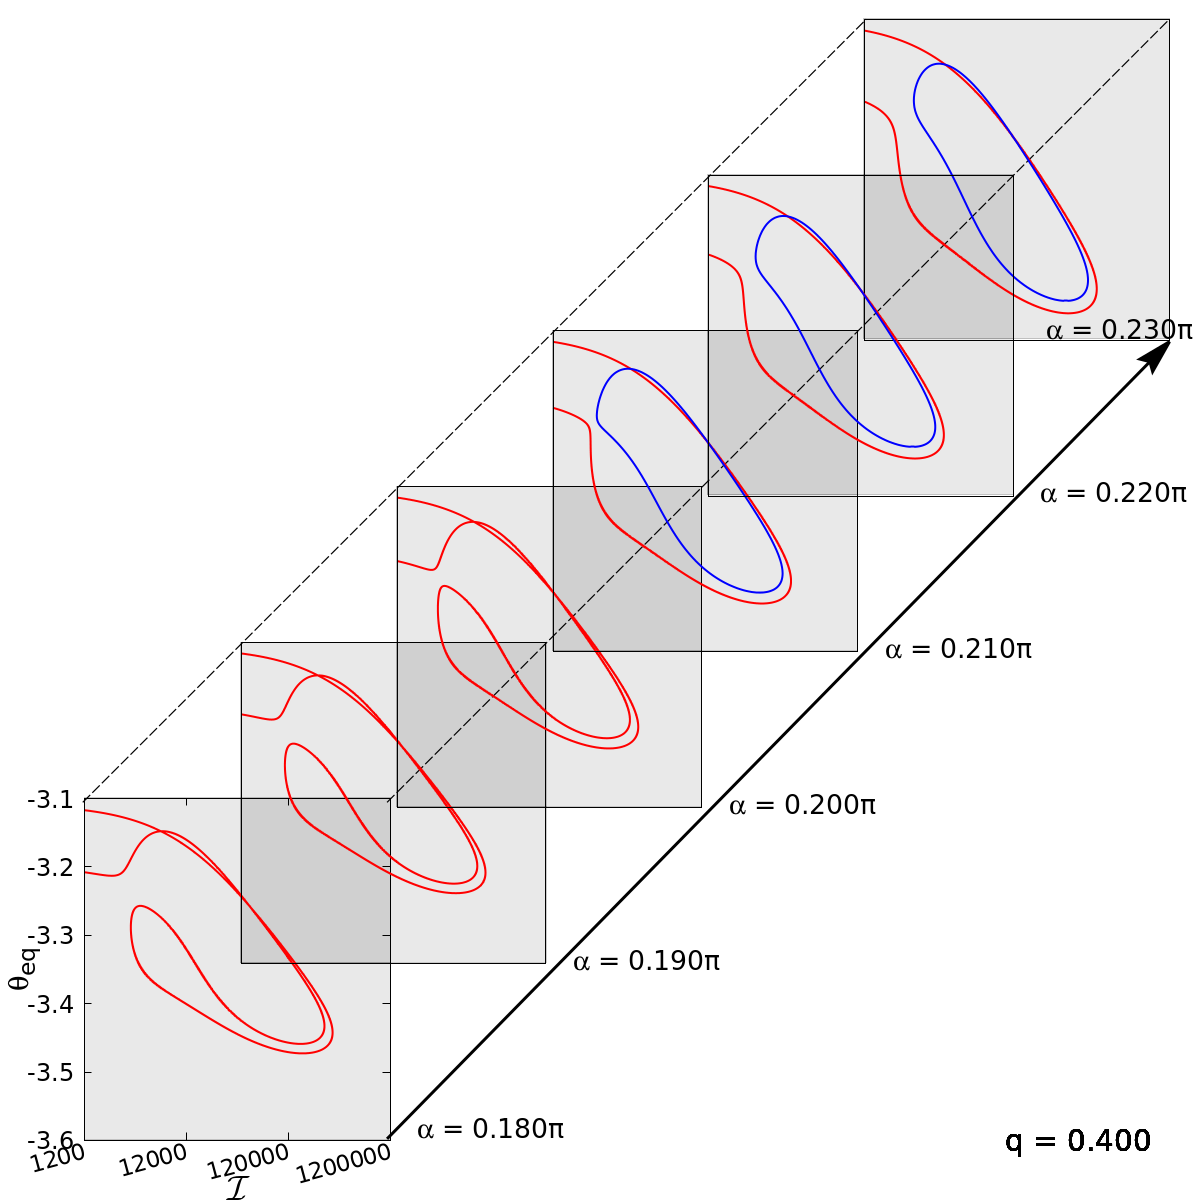
\includegraphics[width=0.65\textwidth]{plots/RESLT_animation_varying_alpha_q_0.400_step_rescale_FSI_slides/elastic_beam_I_theta_q_0.400_alpha_5.png}
			\end{center}
			%	\setlength{\abovecaptionskip}{-0.5 cm}
		\end{figure}	\vspace{-7.5cm}
	\begin{figure}[htb]
	\raggedright
	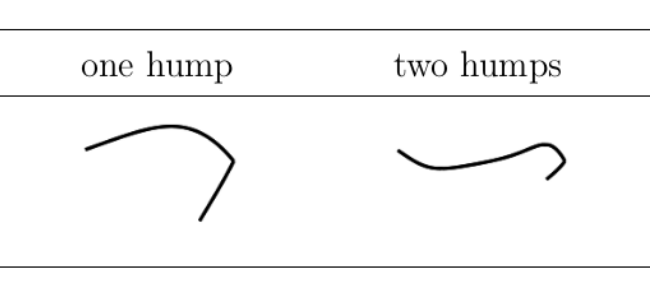
\includegraphics[width=0.4\textwidth]{plots/two_deformations.png}
	%	\setlength{\abovecaptionskip}{-0.5 cm}
\end{figure}
		\vspace{-0.3cm}  % Reduce space below the image
		
		% Bullet-point list under the image
		\begin{tikzpicture}[remember picture, overlay]
			\node[anchor=north west, text=black, font=\scriptsize\bfseries]
			at ([xshift=1.25cm,yshift=-2.91cm]current page.north west) {outer loop};
		\end{tikzpicture}
		\begin{tikzpicture}[remember picture, overlay]
			\node[anchor=north west, text=black, font=\scriptsize\bfseries]
			at ([xshift=3.45cm,yshift=-2.91cm]current page.north west) {inner loop};
		\end{tikzpicture}
	\end{overlayarea}
\end{frame}


%%%%%%%%%%%%%%%%%%%%%%%%%%%%%%%%%%%%%%%%%%%%%%%%%%%%%%%%%%%%%%%%%%%%%%


\begin{frame}
	\frametitle{Results (larger $q$): it gets even more messy.}
	\begin{overlayarea}{\textwidth}{\textheight}\vspace{-0.3cm}
		\begin{figure}[htb]
			\begin{center}
				% specify width as 80% of the width of the text on the page
				% we can also specify a width in centimetres, e.g. [width=8cm]
				\includegraphics[width=0.65\textwidth]{plots/elastic_beam_I_theta_q_0.452_alpha_restart3.png}
			\end{center}
			%	\setlength{\abovecaptionskip}{-0.5 cm}
		\end{figure}\vspace{-0.3cm}
		\bi
		\item More disconnected loops.
		\ei 
		%\selectfont \fontsize{10}{15}\selectfont
	\end{overlayarea}
\end{frame}

%%%%%%%%%%%%%%%%%%%%%%%%%%%%%%%%%%%%%%%%%%%%%%%%%%%%%%%%%%%%%%%%%%%%%%


\begin{frame}
	\frametitle{\mbox{}}
	\begin{overlayarea}{\textwidth}{\textheight}\vspace{2.2cm}
	\Huge\centering What about the stability of these solutions?
	\end{overlayarea}
\end{frame}

%%%%%%%%%%%%%%%%%%%%%%%%%%%%%%%%%%%%%%%%%%%%%%%%%%%%%%%%%%%%%%%%%%%%%%


\begin{frame}
	\frametitle{Linear stability}
	\begin{overlayarea}{\textwidth}{\textheight}\vspace{-0.3cm}
		Reminder: base state is dependent of time:
		\begin{equation*}
			\colorbox{yellow}{$\bm{X}(t)=\bar{\bm{X}}(\alert{t})+\epsilon \hat{\bm{X}}(t)$.}
		\end{equation*}
		\begin{equation*}
			\bm{E}(\bm{X})=\bm{E}(\bar{\bm{X}}+\epsilon \hat{\bm{X}})=\bm{E}(\bar{\bm{X}})+\epsilon \Big(\frac{\partial \bm{E}}{\partial \bm{X}}\Big|_{\bm{X}=\bar{\bm{X}}}\hat{\bm{X}}+\frac{\partial \bm{E}}{\partial \dot{\bm{X}}}\Big|_{\bm{X}=\bar{\bm{X}}}\dot{\hat{\bm{X}}}\Big)+o(\epsilon).
		\end{equation*}
		Since $\bm{E}(\bar{\bm{X}}(t))=\bm{0}$, we have 
		\begin{equation*}
			\frac{\partial \bm{E}}{\partial \bm{X}}\Big|_{\bm{X}=\bar{\bm{X}}}\hat{\bm{X}}+\frac{\partial \bm{E}}{\partial \dot{\bm{X}}}\Big|_{\bm{X}=\bar{\bm{X}}}\dot{\hat{\bm{X}}}=\bm{0}.
		\end{equation*}
		\begin{equation*}
			\bm{\mathcal{J}}\hat{\bm{X}}+\bm{\mathcal{M}}\dot{\hat{\bm{X}}}=\bm{0},
		\end{equation*}
		where $\bm{\mathcal{J}}=\frac{\partial \bm{E}}{\partial \bm{X}}\Big|_{\bm{X}=\bar{\bm{X}}}$ and $\bm{\mathcal{M}}=\frac{\partial \bm{E}}{\partial \dot{\bm{X}}}\Big|_{\bm{X}=\bar{\bm{X}}}$.
		\begin{equation*}
			(\lambda\bm{\mathcal{M}}+\bm{\mathcal{J}})\bm{v}=\bm{0}.
		\end{equation*}
		%\selectfont \fontsize{10}{15}\selectfont
	\end{overlayarea}
\end{frame}

%%%%%%%%%%%%%%%%%%%%%%%%%%%%%%%%%%%%%%%%%%%%%%%%%%%%%%%%%%%%%%%%%%%%%%


\begin{frame}
	\frametitle{Linear stability}
	\begin{overlayarea}{\textwidth}{\textheight}\vspace{-0.3cm}
			Reminder: base state is dependent of time:
			\begin{equation*}
			\colorbox{yellow}{$\bm{X}(t)=\bar{\bm{X}}(\alert{t})+\epsilon \hat{\bm{X}}(\xi,t)$.}
		\end{equation*}
		\begin{equation*}
			\bm{E}(\bm{X})=\bm{E}(\bar{\bm{X}}+\epsilon \hat{\bm{X}})=\bm{E}(\bar{\bm{X}})+\epsilon \Big(\frac{\partial \bm{E}}{\partial \bm{X}}\Big|_{\bm{X}=\bar{\bm{X}}}\hat{\bm{X}}+\frac{\partial \bm{E}}{\partial \dot{\bm{X}}}\Big|_{\bm{X}=\bar{\bm{X}}}\dot{\hat{\bm{X}}}\Big)+o(\epsilon).
		\end{equation*}
		Since $\bm{E}(\bar{\bm{X}}(t))=\bm{0}$, we have 
		\begin{equation*}
			\frac{\partial \bm{E}}{\partial \bm{X}}\Big|_{\bm{X}=\bar{\bm{X}}}\hat{\bm{X}}+\frac{\partial \bm{E}}{\partial \dot{\bm{X}}}\Big|_{\bm{X}=\bar{\bm{X}}}\dot{\hat{\bm{X}}}=\bm{0}.
		\end{equation*}
		\begin{equation*}
			\bm{\mathcal{J}}\hat{\bm{X}}+\bm{\mathcal{M}}\dot{\hat{\bm{X}}}=\bm{0},
		\end{equation*}
		\colorbox{yellow}{but $\bm{\mathcal{J}}$ and $\bm{\mathcal{M}}$ are both independent of time.}
		\begin{equation*}
			(\lambda\bm{\mathcal{M}}+\bm{\mathcal{J}})\bm{v}=\bm{0}.
		\end{equation*}
	$\Rightarrow$ Solve the standard eigenproblem. 
		%\selectfont \fontsize{10}{15}\selectfont
	\end{overlayarea}
\end{frame}

%%%%%%%%%%%%%%%%%%%%%%%%%%%%%%%%%%%%%%%%%%%%%%%%%%%%%%%%%%%%%%%%%%%%%%


\begin{frame}
	\frametitle{Linear stability}
	% Define an overlay area that covers the full slide
	\begin{overlayarea}{\textwidth}{\textheight}
		\vspace{-0.3cm}  % Reduce space above image		
		\begin{figure}[htb]
			\begin{center}
				% specify width as 80% of the width of the text on the page
				% we can also specify a width in centimetres, e.g. [width=8cm]
				\includegraphics[width=0.9\textwidth]{plots/RESLT_q_0.40_alpha_0.230pi_plot_step_refine2_new_recale_FSI_slides/combine_elastic_beam_I_theta_q_0.40_alpha_0.230pi_initial_-4.80_refine2_new_not_log_18.png}
			\end{center}
			%	\setlength{\abovecaptionskip}{-0.5 cm}
		\end{figure}	
		\vspace{-0.3cm}  % Reduce space below the image
		
		% Bullet-point list under the image
		\begin{tikzpicture}[remember picture, overlay]
			\node[anchor=north west, text=black, font=\small\bfseries]
			at ([xshift=0.15cm,yshift=-1.9cm]current page.north west) {stable};
		\end{tikzpicture}
		\begin{tikzpicture}[remember picture, overlay]
			\node[anchor=north west, text=black, font=\small\bfseries]
			at ([xshift=0.15cm,yshift=-2.9cm]current page.north west) {unstable};
		\end{tikzpicture}
	\end{overlayarea}
\end{frame}


%%%%%%%%%%%%%%%%%%%%%%%%%%%%%%%%%%%%%%%%%%%%%%%%%%%%%%%%%%%%%%%%%%%%%%


\begin{frame}
	\frametitle{Linear stability}
	% Define an overlay area that covers the full slide
	\begin{overlayarea}{\textwidth}{\textheight}
		\vspace{-0.3cm}  % Reduce space above image		
		\begin{figure}[htb]
			\begin{center}
				% specify width as 80% of the width of the text on the page
				% we can also specify a width in centimetres, e.g. [width=8cm]
				\includegraphics[width=0.9\textwidth]{plots/RESLT_q_0.40_alpha_0.230pi_plot_step_refine2_new_recale_FSI_slides/combine_elastic_beam_I_theta_q_0.40_alpha_0.230pi_initial_-4.80_refine2_15_new_not_log_dash_line.png}
			\end{center}
			%	\setlength{\abovecaptionskip}{-0.5 cm}
		\end{figure}	
		\vspace{-0.3cm}  % Reduce space below the image
		\bi
		\item Upper branch (stable): no positive eigenvalue.\vspace{-1.1cm}
		\item Lower branch (unstable): one positive eigenvalue.{\fontsize{60}{1}\selectfont \textcolor{red}{\checkmark}}
		\ei
		% Bullet-point list under the image
		\begin{tikzpicture}[remember picture, overlay]
			\node[anchor=north west, text=black, font=\small\bfseries]
			at ([xshift=0.15cm,yshift=-1.9cm]current page.north west) {stable};
		\end{tikzpicture}
		\begin{tikzpicture}[remember picture, overlay]
			\node[anchor=north west, text=black, font=\small\bfseries]
			at ([xshift=0.15cm,yshift=-2.9cm]current page.north west) {unstable}; 
		\end{tikzpicture}
	\end{overlayarea}
\end{frame}


%%%%%%%%%%%%%%%%%%%%%%%%%%%%%%%%%%%%%%%%%%%%%%%%%%%%%%%%%%%%%%%%%%%%%%


\begin{frame}
	\frametitle{Linear stability}
	% Define an overlay area that covers the full slide
	\begin{overlayarea}{\textwidth}{\textheight}
		\vspace{-0.3cm}  % Reduce space above image		
		\begin{figure}[htb]
			\begin{center}
				% specify width as 80% of the width of the text on the page
				% we can also specify a width in centimetres, e.g. [width=8cm]
				\includegraphics[width=0.9\textwidth]{plots/RESLT_q_0.400_alpha_0.180pi_plot_initial_step_refine2_new_recale_FSI_slides/initial_combine_elastic_beam_I_theta_q_0.400_alpha_0.180pi_initial_-4.80_refine2_new_5.png}
			\end{center}
			%	\setlength{\abovecaptionskip}{-0.5 cm}
		\end{figure}	
		\vspace{-0.3cm}  % Reduce space below the image
		\bi
		\item Smaller $\alpha$.
		\ei
		% Bullet-point list under the image
		\begin{tikzpicture}[remember picture, overlay]
			\node[anchor=north west, text=black, font=\small\bfseries]
			at ([xshift=0.15cm,yshift=-1.5cm]current page.north west) {stable};
		\end{tikzpicture}
		\begin{tikzpicture}[remember picture, overlay]
			\node[anchor=north west, text=black, font=\small\bfseries]
			at ([xshift=0.15cm,yshift=-2.6cm]current page.north west) {unstable};
		\end{tikzpicture}
	\end{overlayarea}
\end{frame}


%%%%%%%%%%%%%%%%%%%%%%%%%%%%%%%%%%%%%%%%%%%%%%%%%%%%%%%%%%%%%%%%%%%%%%

\begin{frame}
	\frametitle{Linear stability}
	% Define an overlay area that covers the full slide
	\begin{overlayarea}{\textwidth}{\textheight}
		\vspace{-0.3cm}  % Reduce space above image		
		\begin{figure}[htb]
			\begin{center}
				% specify width as 80% of the width of the text on the page
				% we can also specify a width in centimetres, e.g. [width=8cm]
				\includegraphics[width=0.9\textwidth]{plots/RESLT_q_0.400_alpha_0.180pi_plot_initial_step_refine2_new_recale_FSI_slides/initial_combine_elastic_beam_I_theta_q_0.400_alpha_0.180pi_initial_-4.80_refine2_new_dash_line.png}
			\end{center}
			%	\setlength{\abovecaptionskip}{-0.5 cm}
		\end{figure}	
		\vspace{-0.3cm}  % Reduce space below the image
		\bi
		\item Smaller $\alpha$.\vspace{-1cm}
		\item More positive eigenvalues $\Rightarrow$ Only one stable branch!$\,${\fontsize{60}{1}\selectfont \textcolor{red}{\textbf{!}}}	
		\ei
		% Bullet-point list under the image
		\begin{tikzpicture}[remember picture, overlay]
			\node[anchor=north west, text=black, font=\small\bfseries]
			at ([xshift=0.15cm,yshift=-1.5cm]current page.north west) {stable};
		\end{tikzpicture}
		\begin{tikzpicture}[remember picture, overlay]
			\node[anchor=north west, text=black, font=\small\bfseries]
			at ([xshift=0.15cm,yshift=-2.6cm]current page.north west) {unstable};
		\end{tikzpicture}
	\end{overlayarea}
\end{frame}


%%%%%%%%%%%%%%%%%%%%%%%%%%%%%%%%%%%%%%%%%%%%%%%%%%%%%%%%%%%%%%%%%%%%%%

\begin{frame}
	\frametitle{\mbox{}}
	\begin{overlayarea}{\textwidth}{\textheight}\vspace{2cm}
		\huge\centering Transition from non-rotating to rotating solutions:\\A Sniper bifurcation
	\end{overlayarea}
\end{frame}

%%%%%%%%%%%%%%%%%%%%%%%%%%%%%%%%%%%%%%%%%%%%%%%%%%%%%%%%%%%%%%%%%%%%%%


\begin{frame}
	\frametitle{Region of solutions}
	\hspace*{-1cm}\begin{overlayarea}{\textwidth}{\textheight}\vspace{-0.5cm}
		\foreach \index in {1,...,1} % 490}
	{\pgfmathsetmacro\picnumber{int(\index-1)}	
		\only<\index>{% FRAME: \index  \ \picnumber	
			\begin{center}	
				\includegraphics<\index>[width=1.2\textwidth]{plots/plots_shape_alpha_22.5000000_new2/I_0.0003000_q_0.300_alpha_22.5000000_initial_-4.80_element_20_\picnumber.png}	
			\end{center}              	
			%\includegraphics<\index>[width=2\textwidth]{images/warped_disk/fe_soln/resized/frame\picnumber.png}}
		\bi
		\item Grey region: steady orientations for $\mathcal{I}=0$ (rigid).
		\ei	
	}
	%\scalebox{1.0}{\import{\PaperImagePath}{trajectories_Rc=0.5_red_karaoke/frame1.tex}}	
}
\end{overlayarea}
\end{frame}

%%%%%%%%%%%%%%%%%%%%%%%%%%%%%%%%%%%%%%%%%%%%%%%%%%%%%%%%%%%%%%%%%%%%%%


\begin{frame}
	\frametitle{Region of solutions}
	\hspace*{-1cm}\begin{overlayarea}{\textwidth}{\textheight}\vspace{-0.5cm}
		\foreach \index in {1,...,1} % 490}
	{\pgfmathsetmacro\picnumber{int(\index)}	
		\only<\index>{% FRAME: \index  \ \picnumber	
			\begin{center}	
				\includegraphics<\index>[width=1.2\textwidth]{plots/plots_shape_alpha_22.5000000_new2/I_0.0003000_q_0.300_alpha_22.5000000_initial_-4.80_element_20_\picnumber.png}	
			\end{center}              	
			%\includegraphics<\index>[width=2\textwidth]{images/warped_disk/fe_soln/resized/frame\picnumber.png}}
		\bi
		\item Grey region: steady orientations for $\mathcal{I}=0$ (rigid).
		\item Blue line: boundary for $\mathcal{I}=3600$.\\
		\ei	
	}
	%\scalebox{1.0}{\import{\PaperImagePath}{trajectories_Rc=0.5_red_karaoke/frame1.tex}}	
}
\end{overlayarea}
\end{frame}

%%%%%%%%%%%%%%%%%%%%%%%%%%%%%%%%%%%%%%%%%%%%%%%%%%%%%%%%%%%%%%%%%%%%%%

\begin{frame}
	\frametitle{Region of solutions}
	\hspace*{-1cm}\begin{overlayarea}{\textwidth}{\textheight}\vspace{-0.5cm}
		\foreach \index in {1,...,1} % 490}
	{\pgfmathsetmacro\picnumber{int(\index+1)}	
		\only<\index>{% FRAME: \index  \ \picnumber	
			\begin{center}	
				\includegraphics<\index>[width=1.2\textwidth]{plots/plots_shape_alpha_22.5000000_new2/I_0.0003000_q_0.300_alpha_22.5000000_initial_-4.80_element_20_\picnumber.png}	
			\end{center}              	
			%\includegraphics<\index>[width=2\textwidth]{images/warped_disk/fe_soln/resized/frame\picnumber.png}}
\small \bi
	\item For $q$ constant, we have non-rotating solutions for $\alpha<\alpha_{crt}(q,\mathcal{I})$.
	\ei	
	
	}
	%\scalebox{1.0}{\import{\PaperImagePath}{trajectories_Rc=0.5_red_karaoke/frame1.tex}}	
}
\end{overlayarea}
\end{frame}

%%%%%%%%%%%%%%%%%%%%%%%%%%%%%%%%%%%%%%%%%%%%%%%%%%%%%%%%%%%%%%%%%%%%%%

\begin{frame}
	\frametitle{Behaviour for $\alpha<\alpha_{crt}$}
	\hspace*{-1cm}\begin{overlayarea}{\textwidth}{\textheight}\vspace{-0.5cm}
		\foreach \index in {1,...,1} % 490}
	{\pgfmathsetmacro\picnumber{int(\index+2)}	
		\only<\index>{% FRAME: \index  \ \picnumber	
			\begin{center}	
				\includegraphics<\index>[width=1.2\textwidth]{plots/plots_shape_alpha_22.5000000_new2/I_0.0003000_q_0.300_alpha_22.5000000_initial_-4.80_element_20_\picnumber.png}	
			\end{center}              	
			%\includegraphics<\index>[width=2\textwidth]{images/warped_disk/fe_soln/resized/frame\picnumber.png}}
			\small	\bi
		\item For $q$ constant, we have non-rotating solutions for $\alpha<\alpha_{crt}(q,\mathcal{I})$.
		\item Fibre rapidly approach stable steady orientation.
		\ei	
	}
	%\scalebox{1.0}{\import{\PaperImagePath}{trajectories_Rc=0.5_red_karaoke/frame1.tex}}	
}
\end{overlayarea}
\end{frame}

%%%%%%%%%%%%%%%%%%%%%%%%%%%%%%%%%%%%%%%%%%%%%%%%%%%%%%%%%%%%%%%%%%%%%%


\begin{frame}
	\frametitle{Behaviour for $\alpha>\alpha_{crt}$}
	\hspace*{-1cm}\begin{overlayarea}{\textwidth}{\textheight}\vspace{-0.5cm}
		\foreach \index in {1,...,246} % 246}
	{\pgfmathsetmacro\picnumber{int(\index+55)}	
		\only<\index>{% FRAME: \index  \ \picnumber	
			\begin{center}	
				\includegraphics<\index>[width=1.2\textwidth]{plots/plots_shape_alpha_50.0000000_new2/I_0.0003000_q_0.300_alpha_50.0000000_initial_-4.80_element_20_\picnumber.png}	
			\end{center}              	
			%\includegraphics<\index>[width=2\textwidth]{images/warped_disk/fe_soln/resized/frame\picnumber.png}}
		\small \bi
		\item For $q$ constant, we have Jeffery orbits (rotation) for $\alpha>\alpha_{crt}(q,\mathcal{I})$.
		\item Jeffery orbits with period $T$, associated with large-amplitude deformation.
		\ei	
	}
	%\scalebox{1.0}{\import{\PaperImagePath}{trajectories_Rc=0.5_red_karaoke/frame1.tex}}	
}
\end{overlayarea}
\end{frame}



%%%%%%%%%%%%%%%%%%%%%%%%%%%%%%%%%%%%%%%%%%%%%%%%%%%%%%%%%%%%%%%%%%%%%%


\begin{frame}
	\frametitle{Transition: A Sniper bifurcation}
	\begin{overlayarea}{\textwidth}{\textheight}
\vspace{-0.5cm} 
 Transition between rotating and non-rotating solutions:
 \bi
 \item limit point in steady solutions at $\alpha=\alpha_{crt}$;
 \item beyond limit point: periodic solutions with period $T$.
\ei
	\end{overlayarea}
\end{frame}


%%%%%%%%%%%%%%%%%%%%%%%%%%%%%%%%%%%%%%%%%%%%%%%%%%%%%%%%%%%%%%%%%%%%%%

\begin{frame}
	\frametitle{Transition: A Sniper bifurcation}
	\begin{overlayarea}{\textwidth}{\textheight}
		\vspace{-0.5cm} 
		Transition between rotating and non-rotating solutions:
		\bi
		\item limit point in steady solutions at $\alpha=\alpha_{crt}$;
		\item beyond limit point: periodic solutions with period $T$.
		\ei
		$\Rightarrow$ Sniper bifurcation? Would imply 
		\vspace{-0.35cm} 
		\begin{equation*}
			T\propto (\alpha-\alpha_{crt})^{-\frac{1}{2}}.	
		\end{equation*}
		\vspace{-1cm}			
			\begin{figure}[htb]
			\begin{center}
				% specify width as 80% of the width of the text on the page
				% we can also specify a width in centimetres, e.g. [width=8cm]
				\includegraphics[width=0.5\textwidth]{plots/I_0.0003000_q_0.300_initial_-4.80_element_20_T_alpha_plot_new.png}
			\end{center}
			%	\setlength{\abovecaptionskip}{-0.5 cm}
		\end{figure}\vspace{-4.5cm} 
	{\fontsize{60}{1}\selectfont \textcolor{red}{\checkmark}}
	\end{overlayarea}
\end{frame}


%%%%%%%%%%%%%%%%%%%%%%%%%%%%%%%%%%%%%%%%%%%%%%%%%%%%%%%%%%%%%%%%%%%%%%

\begin{frame}
	\frametitle{Summary}
	\begin{overlayarea}{\textwidth}{\textheight}
		\bi
		\item  Elastic boomerang-shaped fibres (opening angle $\alpha$, aspect ratio $q$) in shear flow can either
		\bi
		\item translate while maintaining a \textbf{steady} (!) orientation 
		\ei
		or
		\bi
		\item perform Jeffery orbits while undergoing large flow-induced deformations.
		\ei 
		\item Complicated solution structure with multiple, often disconnected solution branches. Typically, only one branch is stable.
		\item Transition between non-rotating and rotating solutions via a Sniper bifurcation.
		\ei
	\end{overlayarea}
\end{frame}


%%%%%%%%%%%%%%%%%%%%%%%%%%%%%%%%%%%%%%%%%%%%%%%%%%%%%%%%%%%%%%%%%%%%%%


\begin{frame}
	\frametitle{Results: shapes}
	\begin{overlayarea}{\textwidth}{\textheight}
\begin{itemize}
	\item Classify four types of shapes: \vspace{-0.3cm}
	\begin{figure}[htb]
		\begin{center}
			% specify width as 80% of the width of the text on the page
			% we can also specify a width in centimetres, e.g. [width=8cm]
			\includegraphics[width=1\textwidth]{plots/deformations.png}
		\end{center}
		%	\setlength{\abovecaptionskip}{-0.5 cm}
	\end{figure}
	%\selectfont \fontsize{10}{15}\selectfont
\end{itemize}
	\end{overlayarea}
\end{frame}



%%%%%%%%%%%%%%%%%%%%%%%%%%%%%%%%%%%%%%%%%%%%%%%%%%%%%%%%%%%%%%%%%%%%%%

%%%%%%%%%%%%%%%%%%%%%%%%%%%%%%%%%%%%%%%%%%%%%%%%%%%%%%%%%%%%%%%%%%%%%%


\begin{frame}
	\frametitle{Results: shapes}
	\begin{overlayarea}{\textwidth}{\textheight}
		\begin{itemize}
			\item Classify four types of shapes: \vspace{-0.3cm}
			\begin{figure}[htb]
				\begin{center}
					% specify width as 80% of the width of the text on the page
					% we can also specify a width in centimetres, e.g. [width=8cm]
					\includegraphics[width=1\textwidth]{plots/deformations.png}
				\end{center}
				%	\setlength{\abovecaptionskip}{-0.5 cm}
			\end{figure}
			\item Is this Euler buckling?
			\item Is the beam subject to compression?
			%\selectfont \fontsize{10}{15}\selectfont
		\end{itemize}
	\end{overlayarea}
\end{frame}



%%%%%%%%%%%%%%%%%%%%%%%%%%%%%%%%%%%%%%%%%%%%%%%%%%%%%%%%%%%%%%%%%%%%%%


\begin{frame}
	\frametitle{Results: analysis of tensile stress.}
	\begin{overlayarea}{\textwidth}{\textheight}
		\vspace{-0.3cm}
	\begin{itemize}
		\item \small Tensile stress in beam:
		\begin{equation*}
			\sigma(\xi)=\int_0^\xi (\mathbf{f}\cdot\mathbf{e}_t) \left |\frac{\partial \mathbf{R}}{\partial \xi}\right|\,d\xi,
		\end{equation*}
		where $\mathbf{e}_t$ is the unit tangent vector to the surface of the particle. 
	\item \small Therefore, we have 
	\begin{equation*}\small 
		\sigma(\xi)=\left\{
		\begin{aligned}
			\label{eq:4}
			&\int_0^\xi (\mathbf{f}\cdot\mathbf{e}_{t1}) \left |\frac{\partial \mathbf{R}}{\partial \xi}\right|\,d\xi,\quad \xi\in[0,0.5-q];\\
			&-\mathbf{F}_2\cdot\mathbf{e}_{t2}+\int_{0.5-q}^\xi (\mathbf{f}\cdot\mathbf{e}_{t2}) \left |\frac{\partial \mathbf{R}}{\partial \xi}\right|\,d\xi, \quad \xi\in[0.5-q,1].
		\end{aligned}\right.
	\end{equation*}
	\end{itemize}\vspace{-0.4cm}
	\begin{figure}[htb]
	\begin{center}
		% specify width as 80% of the width of the text on the page
		% we can also specify a width in centimetres, e.g. [width=8cm]
		\includegraphics[width=0.55\textwidth]{plots/tensile_boomerang.png}
	\end{center}
	%	\setlength{\abovecaptionskip}{-0.5 cm}
\end{figure}
	\end{overlayarea}
\end{frame}

%%%%%%%%%%%%%%%%%%%%%%%%%%%%%%%%%%%%%%%%%%%%%%%%%%%%%%%%%%%%%%%%%%%%%%

\begin{frame}
	\frametitle{Results: tensile stress.}
	\begin{overlayarea}{\textwidth}{\textheight}
Tensile stress for different shape parameters ($\mathcal{I}=0$).\vspace{-0.2cm}
\begin{figure}[!h]
	\centering
	\subfigure[\tiny $q=0.35,\alpha=0.125\pi$]{
		\begin{minipage}[b]{0.25\textwidth}
			\includegraphics[width=1\textwidth]{plots/sigma_q_0.35_alpha_0.125pi.png} 
		\end{minipage}
		\label{fig:10.a}
	}
	\subfigure[\tiny $q=0.40,\alpha=0.125\pi$]{
		\begin{minipage}[b]{0.25\textwidth}
			\includegraphics[width=1\textwidth]{plots/sigma_q_0.40_alpha_0.125pi.png}
		\end{minipage}
		\label{fig:10.b}
	}
	\subfigure[\tiny $q=0.45,\alpha=0.125\pi$]{
		\begin{minipage}[b]{0.25\textwidth}
			\includegraphics[width=1\textwidth]{plots/sigma_q_0.45_alpha_0.125pi.png}
		\end{minipage}
		\label{fig:10.c}
	}
	\\ 
	\subfigure[\tiny $q=0.35,\alpha=0.25\pi$]{
		\begin{minipage}[b]{0.25\textwidth}
			\includegraphics[width=1\textwidth]{plots/sigma_q_0.35_alpha_0.250pi.png} 
		\end{minipage}
		\label{fig:10.d}
	}
	\subfigure[\tiny $q=0.40,\alpha=0.25\pi$]{
		\begin{minipage}[b]{0.25\textwidth}
			\includegraphics[width=1\textwidth]{plots/sigma_q_0.40_alpha_0.250pi.png}
		\end{minipage}
		\label{fig:10.e}
	}
	\subfigure[\tiny $q=0.45,\alpha=0.25\pi$]{
		\begin{minipage}[b]{0.25\textwidth}
			\includegraphics[width=1\textwidth]{plots/sigma_q_0.45_alpha_0.250pi.png}
		\end{minipage}
		\label{fig:10.f}
	}
\end{figure}
	\end{overlayarea}
\end{frame}

%%%%%%%%%%%%%%%%%%%%%%%%%%%%%%%%%%%%%%%%%%%%%%%%%%%%%%%%%%%%%%%%%%%%%%


\begin{frame}
	\frametitle{Summary}
	\begin{overlayarea}{\textwidth}{\textheight}
	\bi
	\item Consider the case of a single elastic particle in shear flow, as its motion is primarily governed by the background flow, not by interactions with other particles.
	\item Two of the four fixed orientations differ by an angle of $\pi$, but share the same shape.
	\item Initial configuration ($q,\alpha$) plays an important role in deformations.
	\item Four types of deformations observed.
	\item If the short arm is relative small, varying $\alpha$ may cause a bifurcation, creating a new closed loop in the steady orientation vs. FSI coefficient plot.
	\item No matter how complex the curve becomes, it always starts and ends at $\mathcal{I}=0$.
	\ei
	\end{overlayarea}
\end{frame}

%%%%%%%%%%%%%%%%%%%%%%%%%%%%%%%%%%%%%%%%%%%%%%%%%%%%%%%%%%%%%%%%%%%%%%
\begin{frame}
\begin{overlayarea}{\textwidth}{\textheight}
	\frametitle{Bibliography}
	\small
\bibliography{references}
\end{overlayarea}
\end{frame}
%%%%%%%%%%%%%%%%%%%%%%%%%%%%%%%%%%%%%%%%%%%%%%%%%%%%%%%%%%%%%%%%%%%%%%

\begin{frame}
	\frametitle{Brief introduction of finite element method}
	\begin{overlayarea}{\textwidth}{\textheight}
		%\vspace{-0.8cm}
		%	\begin{columns}
			%	\column{.5\textwidth}
			Let us consider a 1D problem: $\mathcal{R}(x;u(x))=0$, for $ x\in [0,1]$ subject to $u(x=0)=g_0, u(x=1)=g_1$.
			\small\bi
			\item Split the solution into two parts (Galerkin method): \vspace{-0.2cm}$$u(x)=u_p(x)+u_h(x)=u_p(x)+\sum^{N-1}_{j=2}U_j\psi_j(x).$$
			($u_p(x=0)=g_0,u_p(x=1)=g_1$; $u_h(x=0)=u_h(x=1)=0$.)
			\item Weak formulation (weak solution satisfies equation almost everywhere of domain): $$r_k(U_2,U_3,...,U_{N-1})=\int^1_0\mathcal{R}\Bigg(u_p(x)+\sum^{N-1}_{j=2}U_j\psi_j(x)\Bigg)\,\psi_k(x)\,dx.$$
			\item Note that $\{U_2,U_3,...U_{N-1}\}$ are the unknowns. 
			\ei
			
			
			%\column{.5\textwidth}
			
			%\end{columns}
		\end{overlayarea}
	\end{frame}
	
	%%%%%%%%%%%%%%%%%%%%%%%%%%%%%%%%%%%%%%%%%%%%%%%%%%%%%%%%%%%%%%%%%%%%%%
	
	
	
	\begin{frame}
		\frametitle{Brief introduction of finite element method}
		\begin{overlayarea}{\textwidth}{\textheight}
			\vspace{-0.2cm}\small	Shape functions: "hat functions".
			$$\psi_j(x)=
			\begin{cases}
				0 & \text{for}\quad x<X_{j-1} \\
				\frac{x-X_{j-1}}{X_{j}-X_{j-1}} & \text{for}\quad X_{j-1}<x<X_{j}\\
				\frac{X_{j+1}-x}{X_{j+1}-X_{j}} & \text{for}\quad X_{j}<x<X_{j+1} \\
				0 & \text{for}\quad x>X_{j+1}
			\end{cases}$$\vspace{-0.6cm}
			\begin{figure}[htb]
				\begin{minipage}[t]{0.49\linewidth}
					\centering
					\includegraphics[scale=0.22]{plots/finite1.png}
				\end{minipage}
				\begin{minipage}[t]{0.49\linewidth}
					\centering
					\includegraphics[scale=0.22]{plots/finite2.png}
				\end{minipage}
			\end{figure}\vspace{-0.2cm}
			\bi
			\item Shape functions satisfy $\psi_j(X_i)=
			\begin{cases}
				1 & \text{if}\quad i=j \\
				0 & \text{for}\quad i\neq j
			\end{cases}.$
			\item Piecewise linear interpolation $v(x)=\sum^N_{j=1} V_j \psi_j(x)$.
			\ei
		\end{overlayarea}
	\end{frame}
	
	%%%%%%%%%%%%%%%%%%%%%%%%%%%%%%%%%%%%%%%%%%%%%%%%%%%%%%%%%%%%%%%%%%%%%%
	
	
	
	\begin{frame}
		\frametitle{Newton method}
		\begin{overlayarea}{\textwidth}{\textheight}
			\vspace{-0.5cm}\small	
			\bi
			\item Set $u_p=g_0\psi_1(x)+g_1\psi_N(x)$ and $\sum^{N-1}_{j=2}U_j\psi_j(x)$.
			\item Provide an initial guess for the unknowns $\{U_2,U_3,...U_{N-1}\}$, denoted as $U_i^{(0)}, i=2,...,N-1.$
			\item Determine the residuals $$r_k^{(0)}=\int^1_0\mathcal{R}\Bigg(u_p(x)+\sum^{N-1}_{j=2}U_j\psi_j(x)\Bigg)\,\psi_k(x)\,dx,\, k=2,...,N-1.$$
			and the entries in the Jacobian matrix $J_{kj}=\frac{\partial r_k}{\partial U_j},\, k,j=2,...,N-1.$
			\item Solve the linear system $\sum^{N-1}_{j=2}J_{kj}\,\delta U_j=-r_k^{(0)},\,k=2,...,N-1.$
			\item Correct the initial guess via $U_j=U_j^{(0)}+\delta U_j,\, j=2,...,N-1.$ 
			\item The finite-element solution is\vspace{-0.2cm} $$u^{(FE)}(x)=g_0\psi_1(x)+g_1\psi_N(x)+\sum^{N-1}_{j=2}U_j\psi_j(x).$$
			\ei
		\end{overlayarea}
	\end{frame}
	
	%%%%%%%%%%%%%%%%%%%%%%%%%%%%%%%%%%%%%%%%%%%%%%%%%%%%%%%%%%%%%%%%%%%%%%

\end{document}


